\section{Experimental Evaluation}
\label{sec:evaluation}

In order to evaluate the security and reliability of our implementation of \name, we conducted a series of experiments

\subsection{Evaluation Focus: Internet Relay}
\label{sec:evaluation:focus}

For the purposes of our evaluation, we make the distinction between two types of relay attacks. In the first type, the adversary redirects the attestation \emph{over the Internet} to another platform that is under his physical control, and therefore in a \emph{different location}. As we explained in Section~\ref{sec:problemStatement:implication}, such relay attack amplifies the adversary's capabilities the most, as he can now attack the attested enclave using physical side-channels, he has unlimited time to launch digital side-channels, or he can wait for the discovery of new attack vectors. 
 
In the second type of relay attack, the adversary redirects the attestation to another \emph{co-located platform}, like another server on the same server rack. In most cases, attestation relay to a co-located platform does not improve the adversary's chances of attacking the enclave, because typically the adversary has similar control over the co-located platform. The only exception is privilege escalation in cases where the adversary has user privileged on the target platform and system privileges on the co-located platform. 

Next, we focus on demonstrating that an inexpensive \name prototype can be configured to prevent the first (and typically more dangerous) type of relay attacks with very strong security and robustness. Later, in Section~\ref{sec:co-located}, we discuss the second type of relay.


\subsection{Experimental Setup}
\label{sec:evaluation:exp}

To demonstrate that \name prevents relay attacks (over the Internet) we performed two types of experiments. First, we tested the legitimate attestation execution with \name and measured the challenge-response latencies between our prototype and the target platform. Second, we \emph{simulated} a relay attack, where the adversary redirects the attestation to another platform.

\begin{figure}[t]
  \centering
    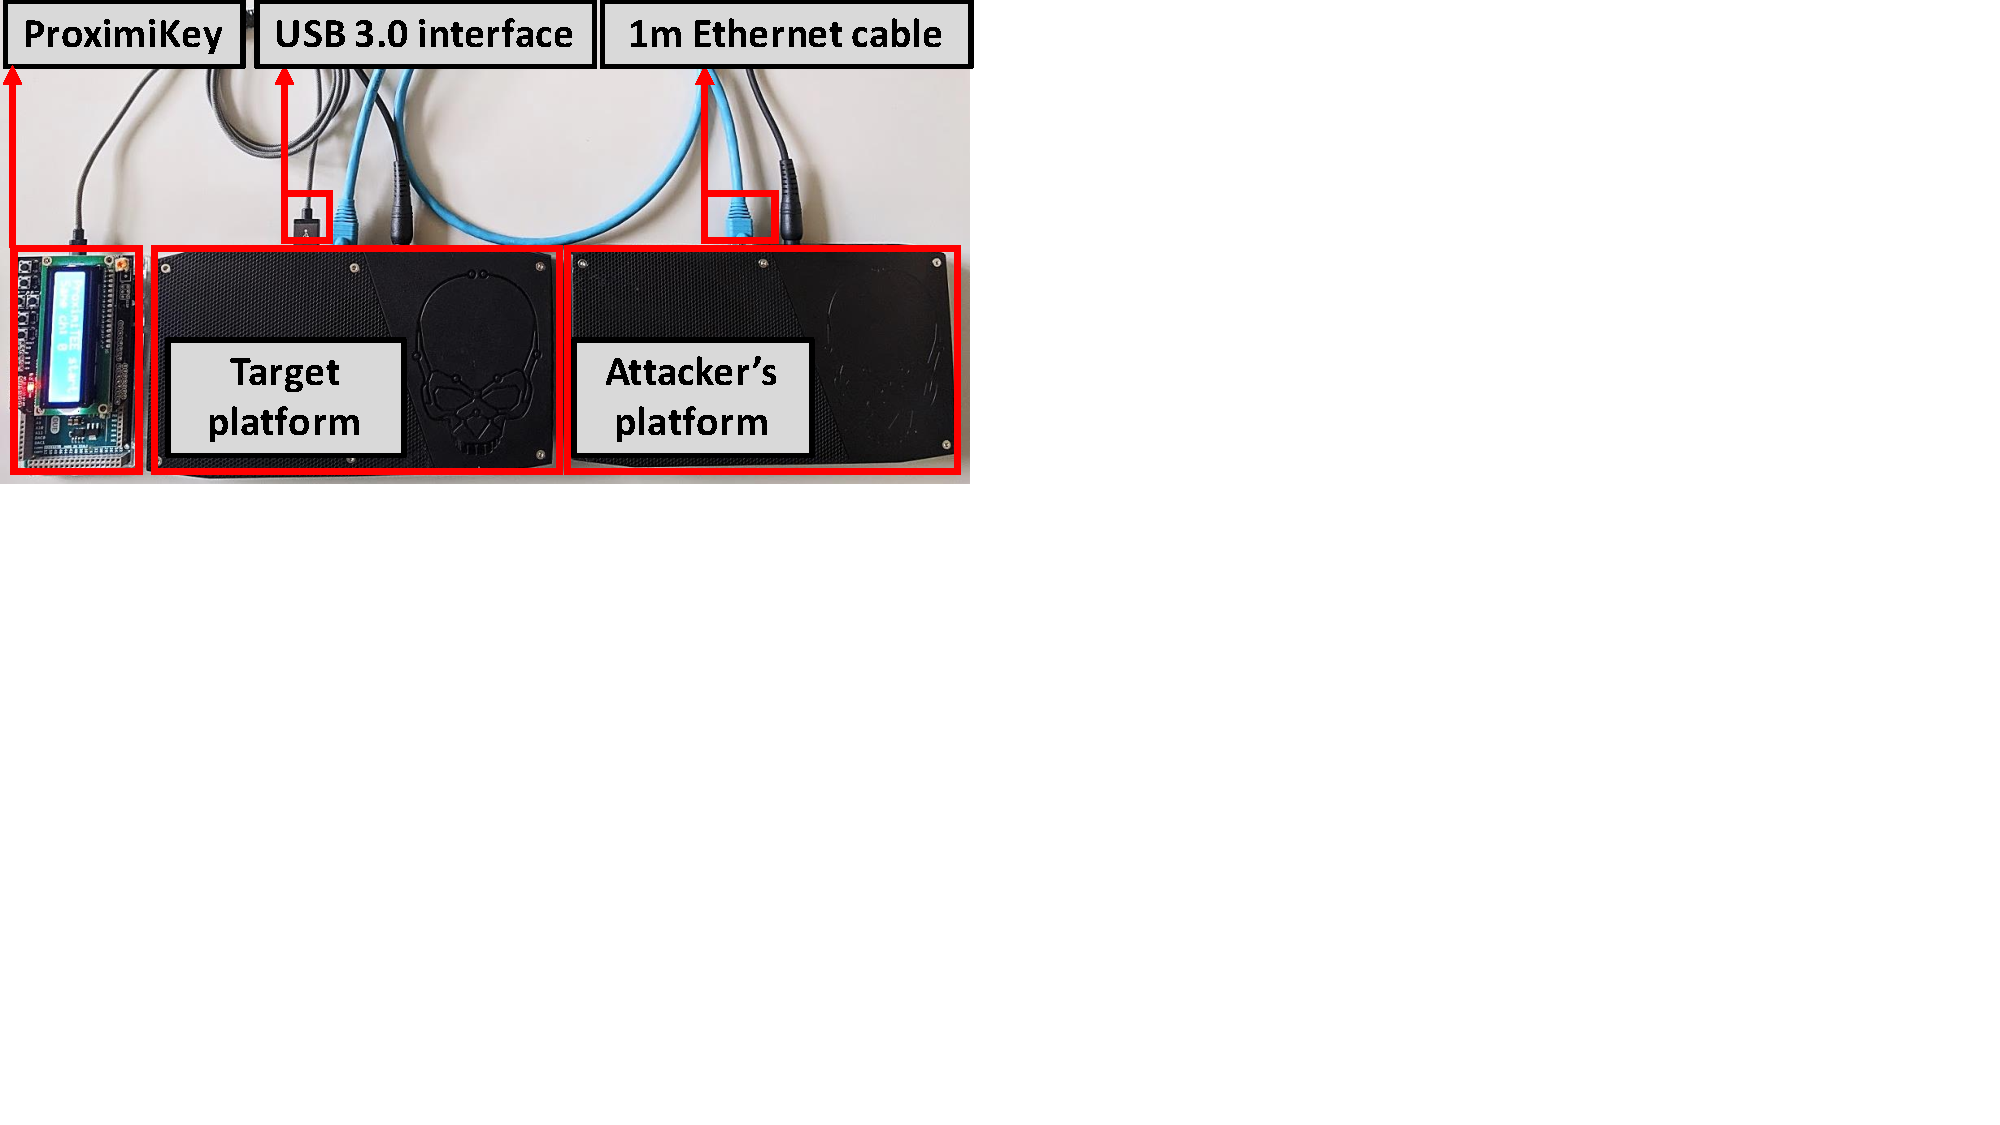
\includegraphics[trim={0 11cm 17cm 0}, clip, width=0.8\linewidth]{chapters/ProximiTEE/figures/Setup2.pdf}
    \caption[\name experimental setup]{\textbf{\name experimental setup} consists of the \device device prototype, the target platform, the attacker's platform and the connection interfaces between them.}

    \label{fig:setup}
\end{figure}

\myparagraph{Assumptions and optimizations}
To consider the best possible case for the adversary, we made several generous assumptions in his favor, when designing our experimental setup and post-processing of our measurement:

\begin{enumerate}
	\item \emph{Single network hop.} Since we do not want to make any assumptions about the precise network path that the relayed attestation needs to travel, we connected the adversary's platform to the target platform via a direct 1-meter Ethernet cable as seen in Figure~\ref{fig:setup}. With such setup, our goal is to simulate the most direct connectivity and the best possible latency that the adversary could achieve in relay attacks that take place over the Internet. In most realistic attacks, the adversary would need to relay the attestation over multiple network hops which increases the round-trip latency significantly. 

	\item \emph{Instant protocol computation.} Since the adversary might have a faster processor on his platform than the one the one we used in our experiments, we simulated an adversary who is able to perform all computations needed for the proximity verification protocol instantly. Instant replies were simulated by fixing the randomness for the challenges and having precomputed responses for that randomness on the attacker's machine.

	\item \emph{Packet forwarding optimizations.} Since the adversary controls the OS on the target platform, he can perform software-based optimizations to reduce the packet forwarding delay. We experimented with several such optimizations. First, we tested the standard \texttt{ping} tool which gave a latency of around $380\ \mu s$ for one-meter Ethernet connection. After that, we used the \texttt{ping} tool in so called flood mode and measured a reduced average network latency of around $153\ \mu s$ (command \texttt{ping -s 300 -af}). Flood mode achieves faster round-trip time as the it forces the OS to fill up the network queue of the kernel. Based on these measurements, we chose to simulate an attacker that fills the kernel's network queues (on both platforms) similar to the flood mode to minimize latency. We also tested other possible OS-level optimizations, but did not observe material reduction in measured latencies, and thus in our experiments we only use the kernel queue filling.
	
	\item \emph{Infinitely fast network interface.} Since the adversary's platform might have a faster network interface hardware than the one used in our experiments, we chose to simulate an adversary that has infinitely fast network interface. In our experimental setup, both the target platform and the adversary's platform have identical network interfaces. We assume (in the favor of the adversary) that the transmission time spent on the wire is negligible and most the the round-trip latency is due to processing the in the network interface. This allows us to simulate an adversary with infinitely fast network interface by first performing latency measurements and then in a post-processing phase cutting down all the measured latencies by half. Note that the target platform's network interface cannot be replaced by the attacker has he does not have physical access to it.
\end{enumerate}

\myparagraph{Experiments}
We conducted our experiments on three SGX platforms: two Intel NUC NUC6i7KYK mini-PCs and one Dell Latitude laptop, all equipped with SGX-enabled Skylake core i7 processors and Ubuntu 16.04 LTS installed on them. To measure latencies we used FX-3's GPIO pins that provides 100 nanosecond level accuracy. We performed a total of $20$ million rounds of the protocol for normal attestations and simulated attacks and measured the challenge-response latencies for each. We measure all of them inside the EZ-USB FX3 code. For cross-validation, we tested the \device with the high precision oscilloscope and witnessed identical timing patterns.


\subsection{Latency Distributions}
\label{sec:evaluation:results}



The histogram in Figure~\ref{graph:instatAttackerHisto} on the left represents the challenge-response latencies in the legitimate proximity verification. The histogram on the right shows latencies in a simulated attack (including a post-processing phase where we reduce the adversary's measured network latencies to half to accommodate the assumption of the attacker's infinitely fast network interface).

As can be seen from Figure~\ref{graph:instatAttackerHisto}, the vast majority of the benign challenge-responses take from $145$ to $250 \mu s$ (average is $185 \mu s$, $95\%$ of samples are in between $150\mu s$ and  $200\mu s$). The vast majority of the round-trip times in the simulated attack take from $200$ to $750$ $\mu s$ (average is 264$\mu s$, $95\%$ of samples are in between 209$\mu s$ and 650 $\mu s$). Hence, the average delay of our simulated adversary is only $80 \mu s$. To put this into perspective, even the highly-optimized network connections between major data centers in the same region exhibit latencies from one millisecond upwards~\cite{agarwal_agarwal_2018} which is one order of magnitude more than in our simulated setup.



\begin{figure}[t]
  \centering
    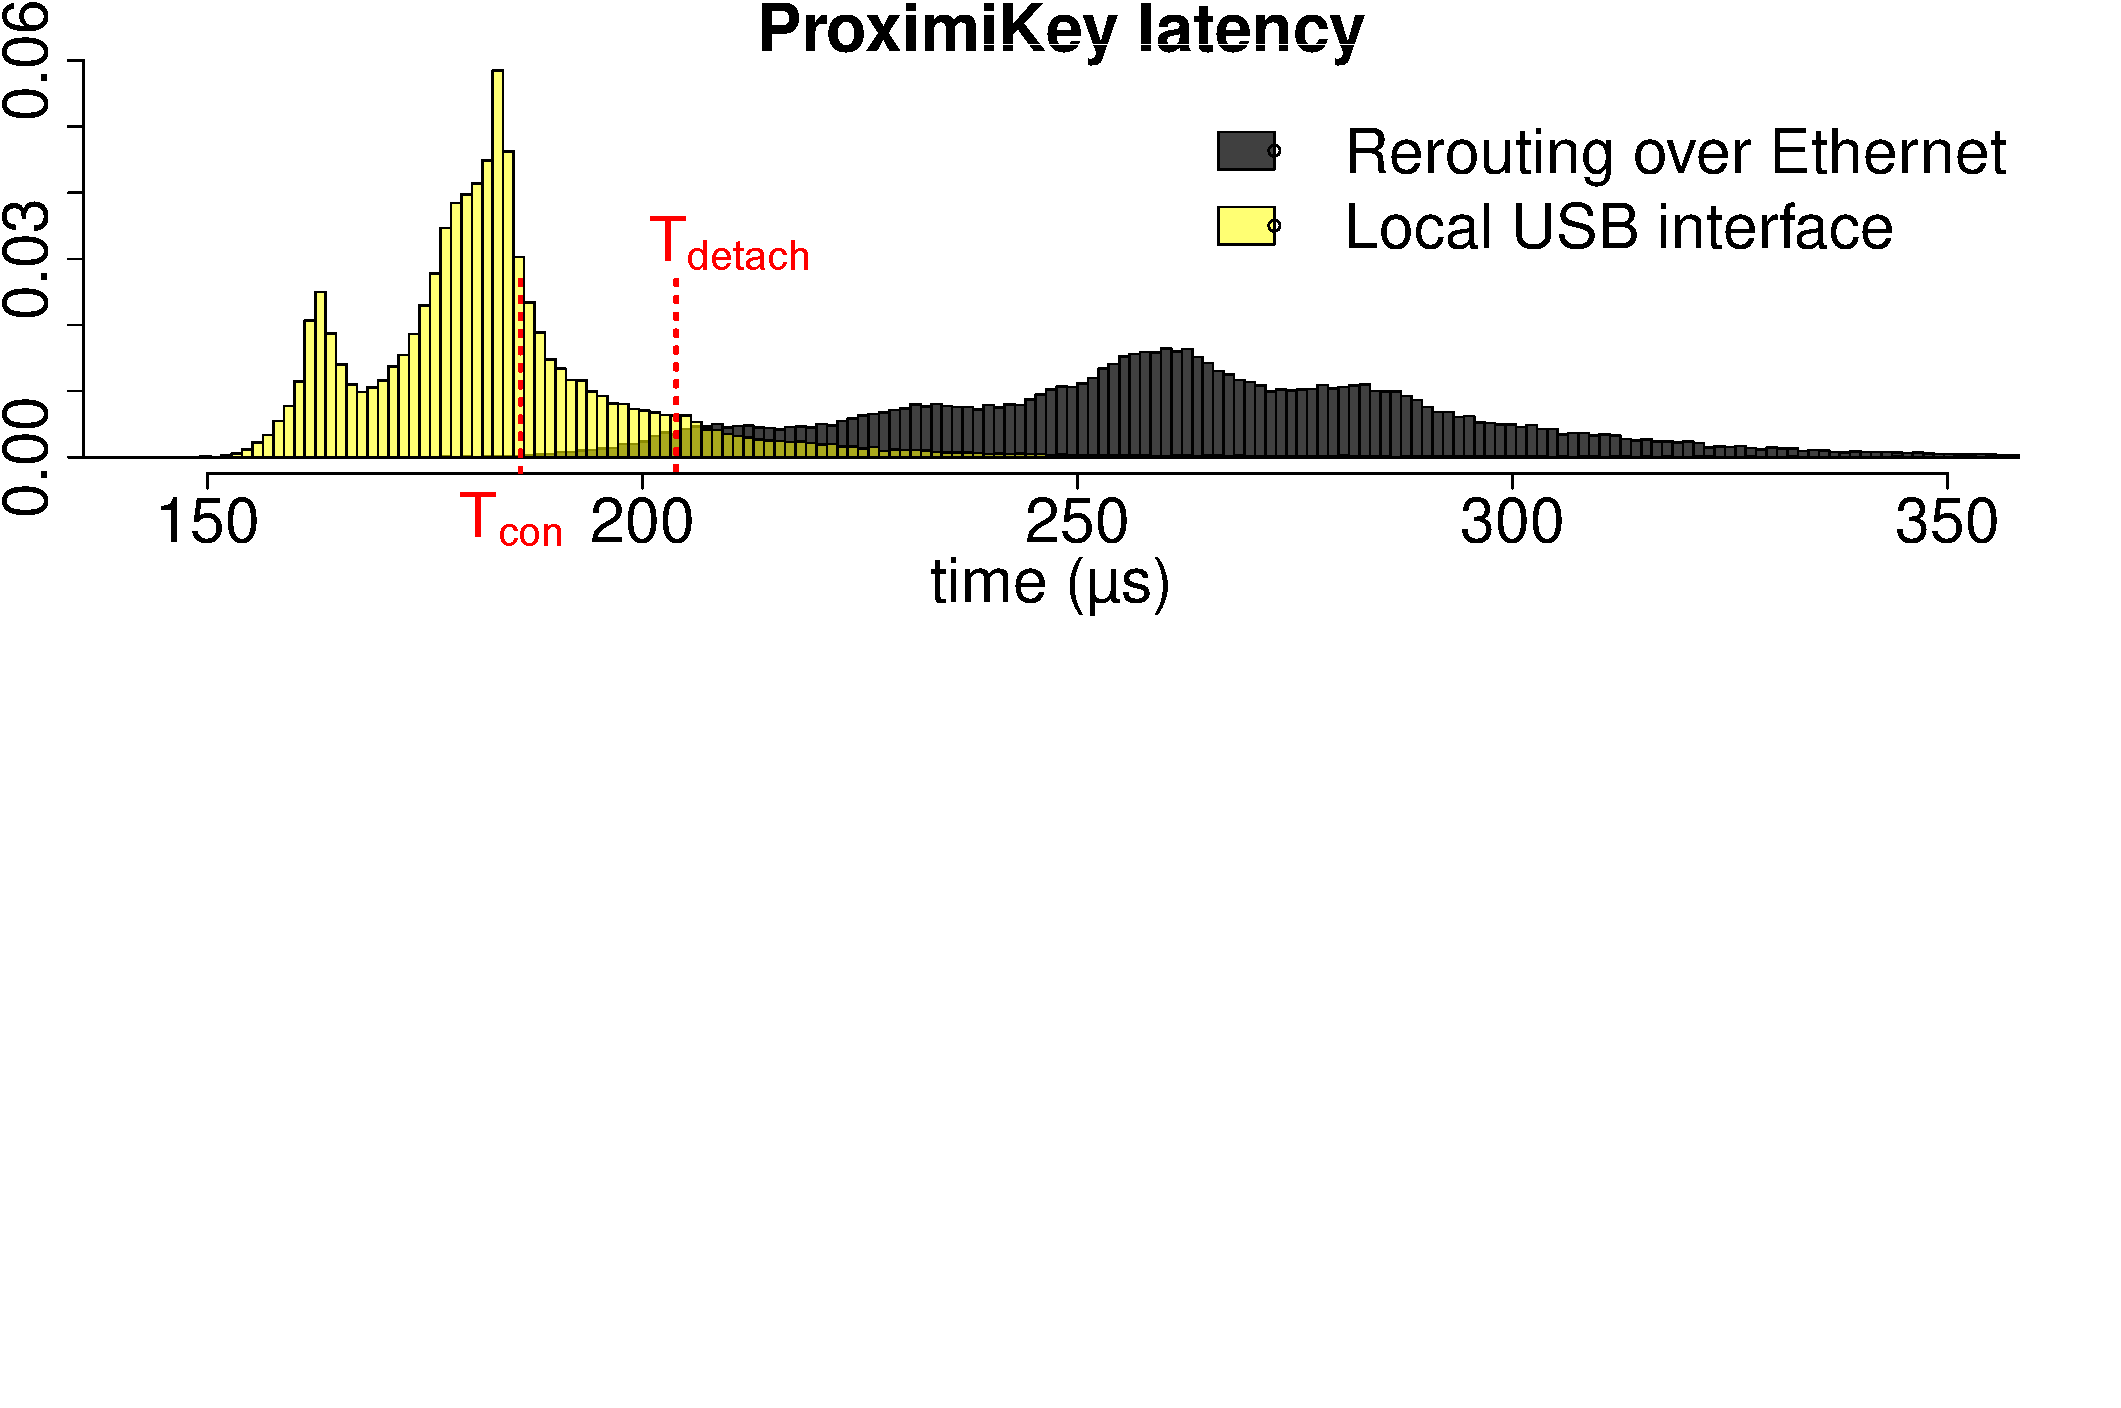
\includegraphics[trim={0 13.4cm 0 0},
    clip,width=\linewidth]{chapters/ProximiTEE/figures/histo.pdf} 
    \caption[Latency distributions]{\textbf{Latency distributions} for legitimate challenge-response rounds (left) and simulated relay attack (right).}
    \label{graph:instatAttackerHisto}
\end{figure}



Besides the latency observed on the side of the embedded device, we measured the time required to compute responses to received challenges on the side of the target platform. We repeated these test on three different SGX platforms and observed results that varied from 6 to 10 $\mu$s. We also measured if the computational load of the target platform influences the time required to compute responses. Under maximum system load (all 8 cores busy), the maximum observed time increased to 20 $\mu$s. Under moderate system load (1 or 2 cores busy), we experience no notable increase in the required computation time. 


\subsection{Initial Proximity Verification Parameters}
\label{sec:evaluation:parameters}

As explained in Section~\ref{sec:systemDesign}, the initial proximity verification is successful when at least fraction $k$ of the $n$ challenge-response latencies are below the threshold \connect.  Now, we explain our strategy for setting these parameters based on the above results.

There are five interlinked parameters that one needs to consider: (i) the legitimate connection latency threshold \connect, (ii) total number of challenge-response rounds $n$, (iii) the fraction $k$, (iv) attacker's success probability $P_{adv}$ that should be negligible, and (v) the legitimate success probability $P_{legit}$ that should be high. We find suitable values for these parameters in the following order:



\newcommand{\mainResultCaption}{\textbf{Distinguishing relay attack.} The attacker's success probability $P_{adv}$ and the legitimate success probability $P_{legit}$ in proximity verification for different number of rounds ($n$) given a fixed $k=0.4$.}


\myparagraph{Finding suitable threshold \connect} Finding a suitable threshold \connect is a non-trivial task. A very low threshold requires a high number of the challenge-response rounds, since the protocol requires at least a fraction $k$ of the observed responses to be less or equal to \connect and a low threshold has very low cumulative probability value in the latency distribution (see Figure~\ref{fig:cdf}). Conversely, a very high threshold value enables some latencies measured during an attack to be classified as legitimate replies, hence increasing the chances of the attacker to break the proximity verification. To address this challenge, we perform a trial over multiple threshold candidates to evaluate their viability.


Figure~\ref{graph:diffTh} shows the legitimate success probability $P_{legit}$ for different number of rounds ($n\in\{10,20,50,100\}$). We iterate through multiple threshold times (\connect$\in\{183\mu s,184\mu s,185\mu s, 186\mu s, 189\mu s\}$), and $186\mu s$ provides high success ratio for different values of $k$ ($P_{legit}=0.(9)_7 77$ $(n=50)$ and $P_{legit}=0.(9)_15 29\ (n=100)$), where $0.(9)_n x$ denotes $n$ times $9$ after the decimal symbol followed by $x$ (e.g., $0.(9)_2 5=0.995$).

We test \connect up until $186 \mu s$ because as can be observed in Figure~\ref{graph:instatAttackerHisto} for these values we observe extremely small occurrences ($1.33\times10^{-3}$) of latency responses during an attacking scenario. It is possible to increment the latency further to improve the success probability, but doing so will start increasing the probability for the attacker as well. 
%
After that, we estimate that any latency value less than or equals to the threshold \connect appears with the cumulative probability of $p_{\mathcal{H}} = \Pr[144\leq x \leq 186] = \sum_{i=144}^{186}\Pr[x=i] = 0.693$ (where $144\ \mu s$ is the smallest latency experienced).

The attacker's success probability for a single round is the cumulative probability sampled from the attacker's distribution (the grey histogram in Figure~\ref{graph:instatAttackerHisto}) $p_\mathcal{A} = \Pr[x \leq 186] = \sum_{i=160}^{183}\Pr[x=i] = 1.33 \times 10^{-4}$.


Now, for both cases (simulated attack and benign case) we can model the complete challenge-response protocol of $n$ rounds as a Bernoulli's trial where we look for at least $kn$ responses within $186\ \mu s$ out of $n$. We can write this cumulative probability as a binomial distribution:
%

\begin{align*}
    \Pr[x \geq nk] = \sum_{i=nk}^n\binom{n}{i} (p)^{i}(1-p)^{n-i};~~\text{where}~ p \in \{p_\mathcal{H}, p_\mathcal{A}\}
\end{align*}

\begin{figure}[t]
  \centering
    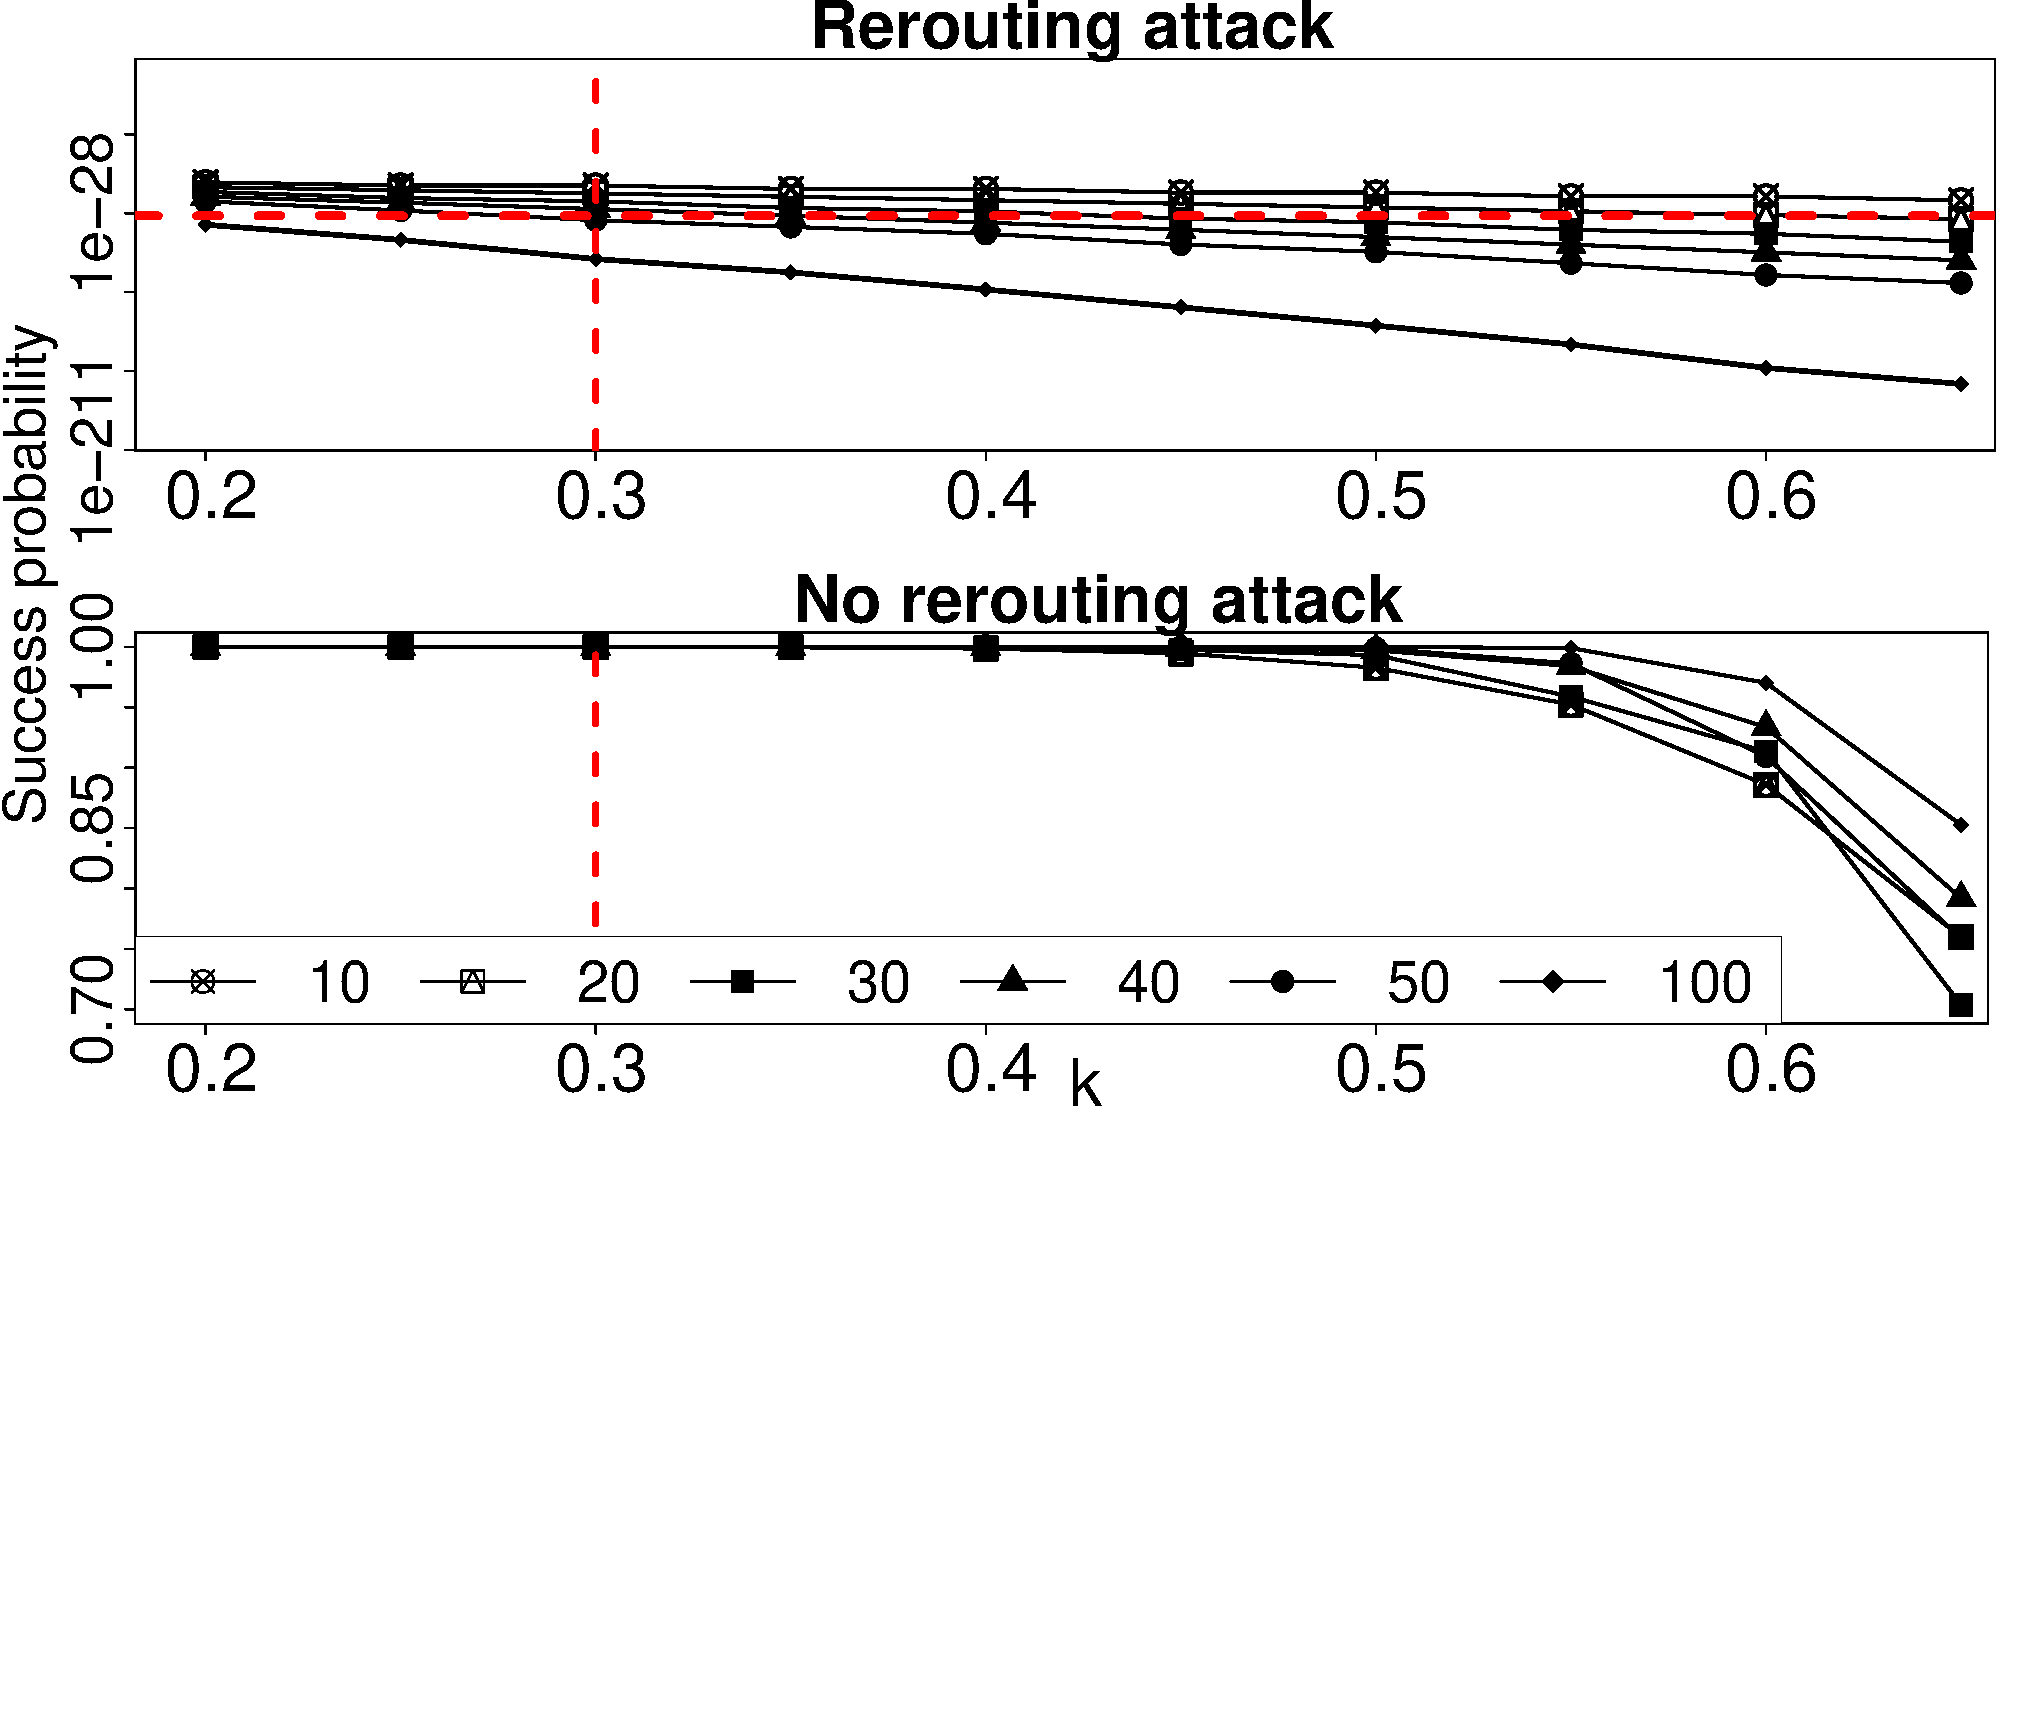
\includegraphics[trim={0 10cm 0 0}, clip, width=\linewidth]{chapters/ProximiTEE/data/fx3_data/round_comp_new.pdf}
    \caption[Finding suitable fraction $k$]{\textbf{Finding suitable fraction $k$.} The graph shows the legitimate enclave's success probability in an ideal scenario and the attacker's success probability in rerouting attack scenario with varying $k$.}
    \label{graph:roundSuccess}
\end{figure}



\begin{figure}[h]
  \centering
    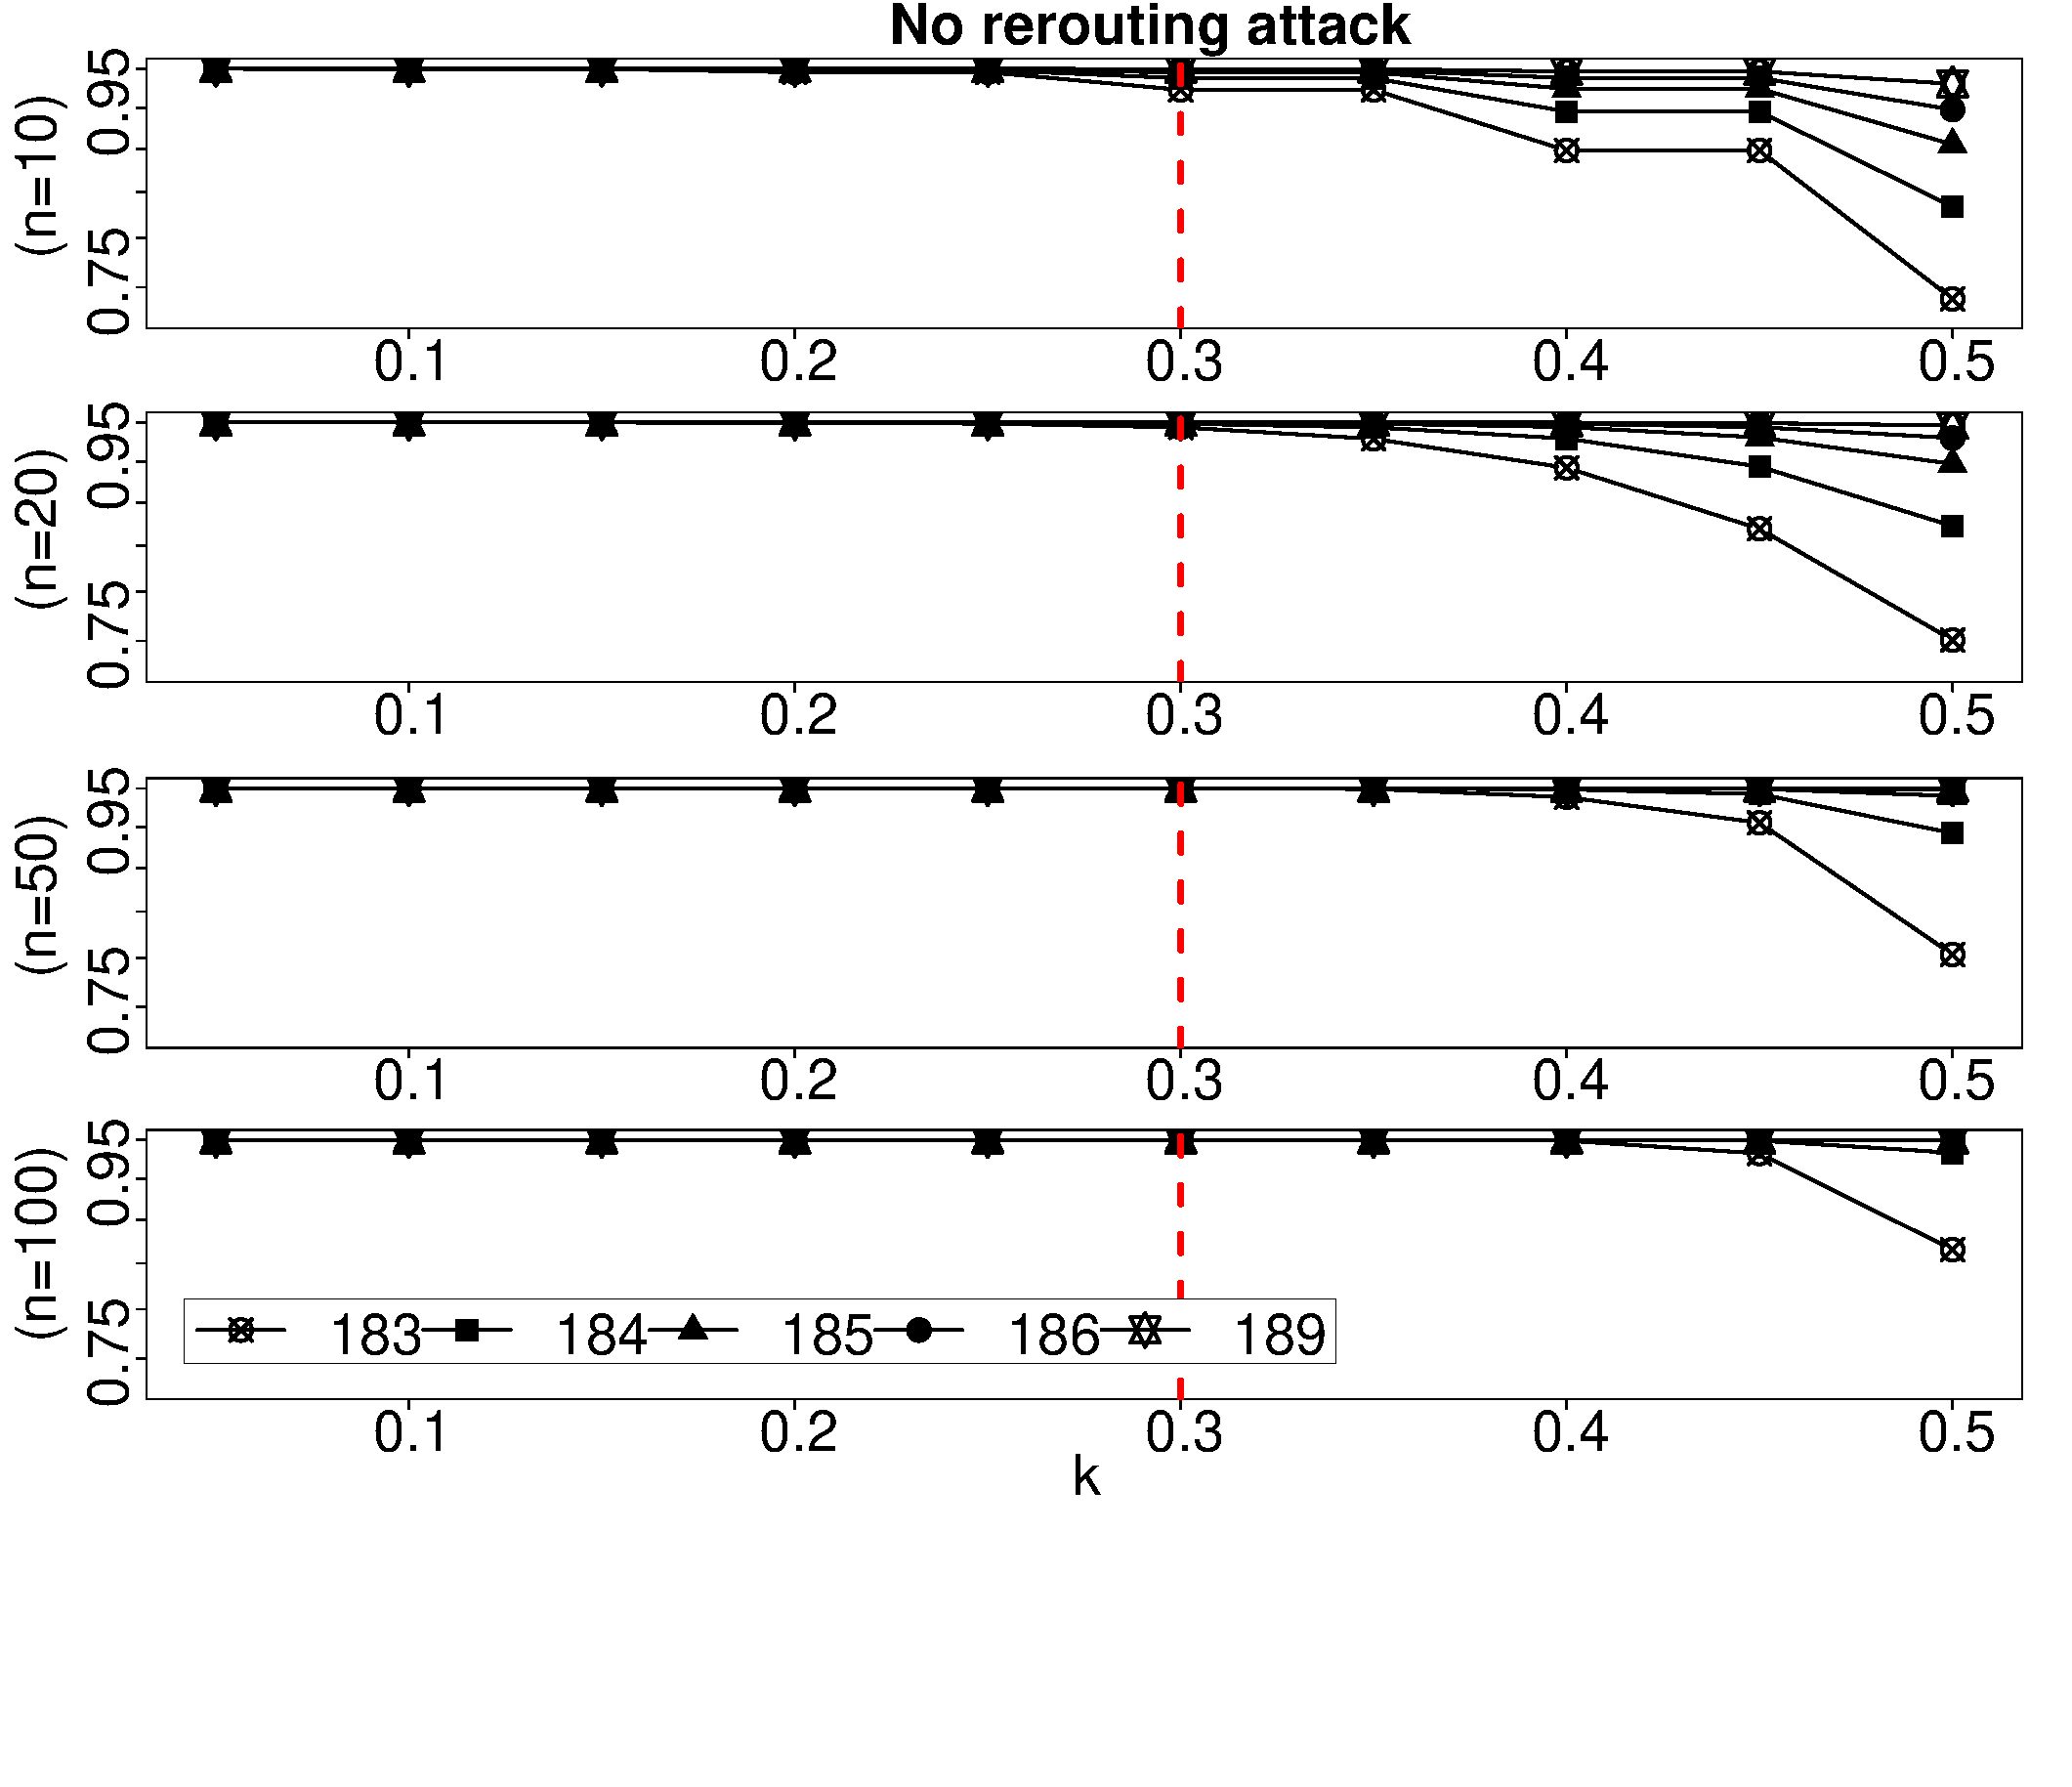
\includegraphics[trim={0 5cm 0 0}, clip, width=\linewidth]{chapters/ProximiTEE/data/fx3_data/timeRound.pdf}
    \caption[Legitimate attestation success probability for different \connect values]{\textbf{Legitimate attestation success probability for different \connect values.} The chosen value \connect $=186\ \mu s$ gives success probability $0.999999977$ for number of trials at least 15 out of $n=50$ rounds when $k=0.3$.}
    \label{graph:diffTh}
\end{figure}


\begin{figure}[h]
  \centering

    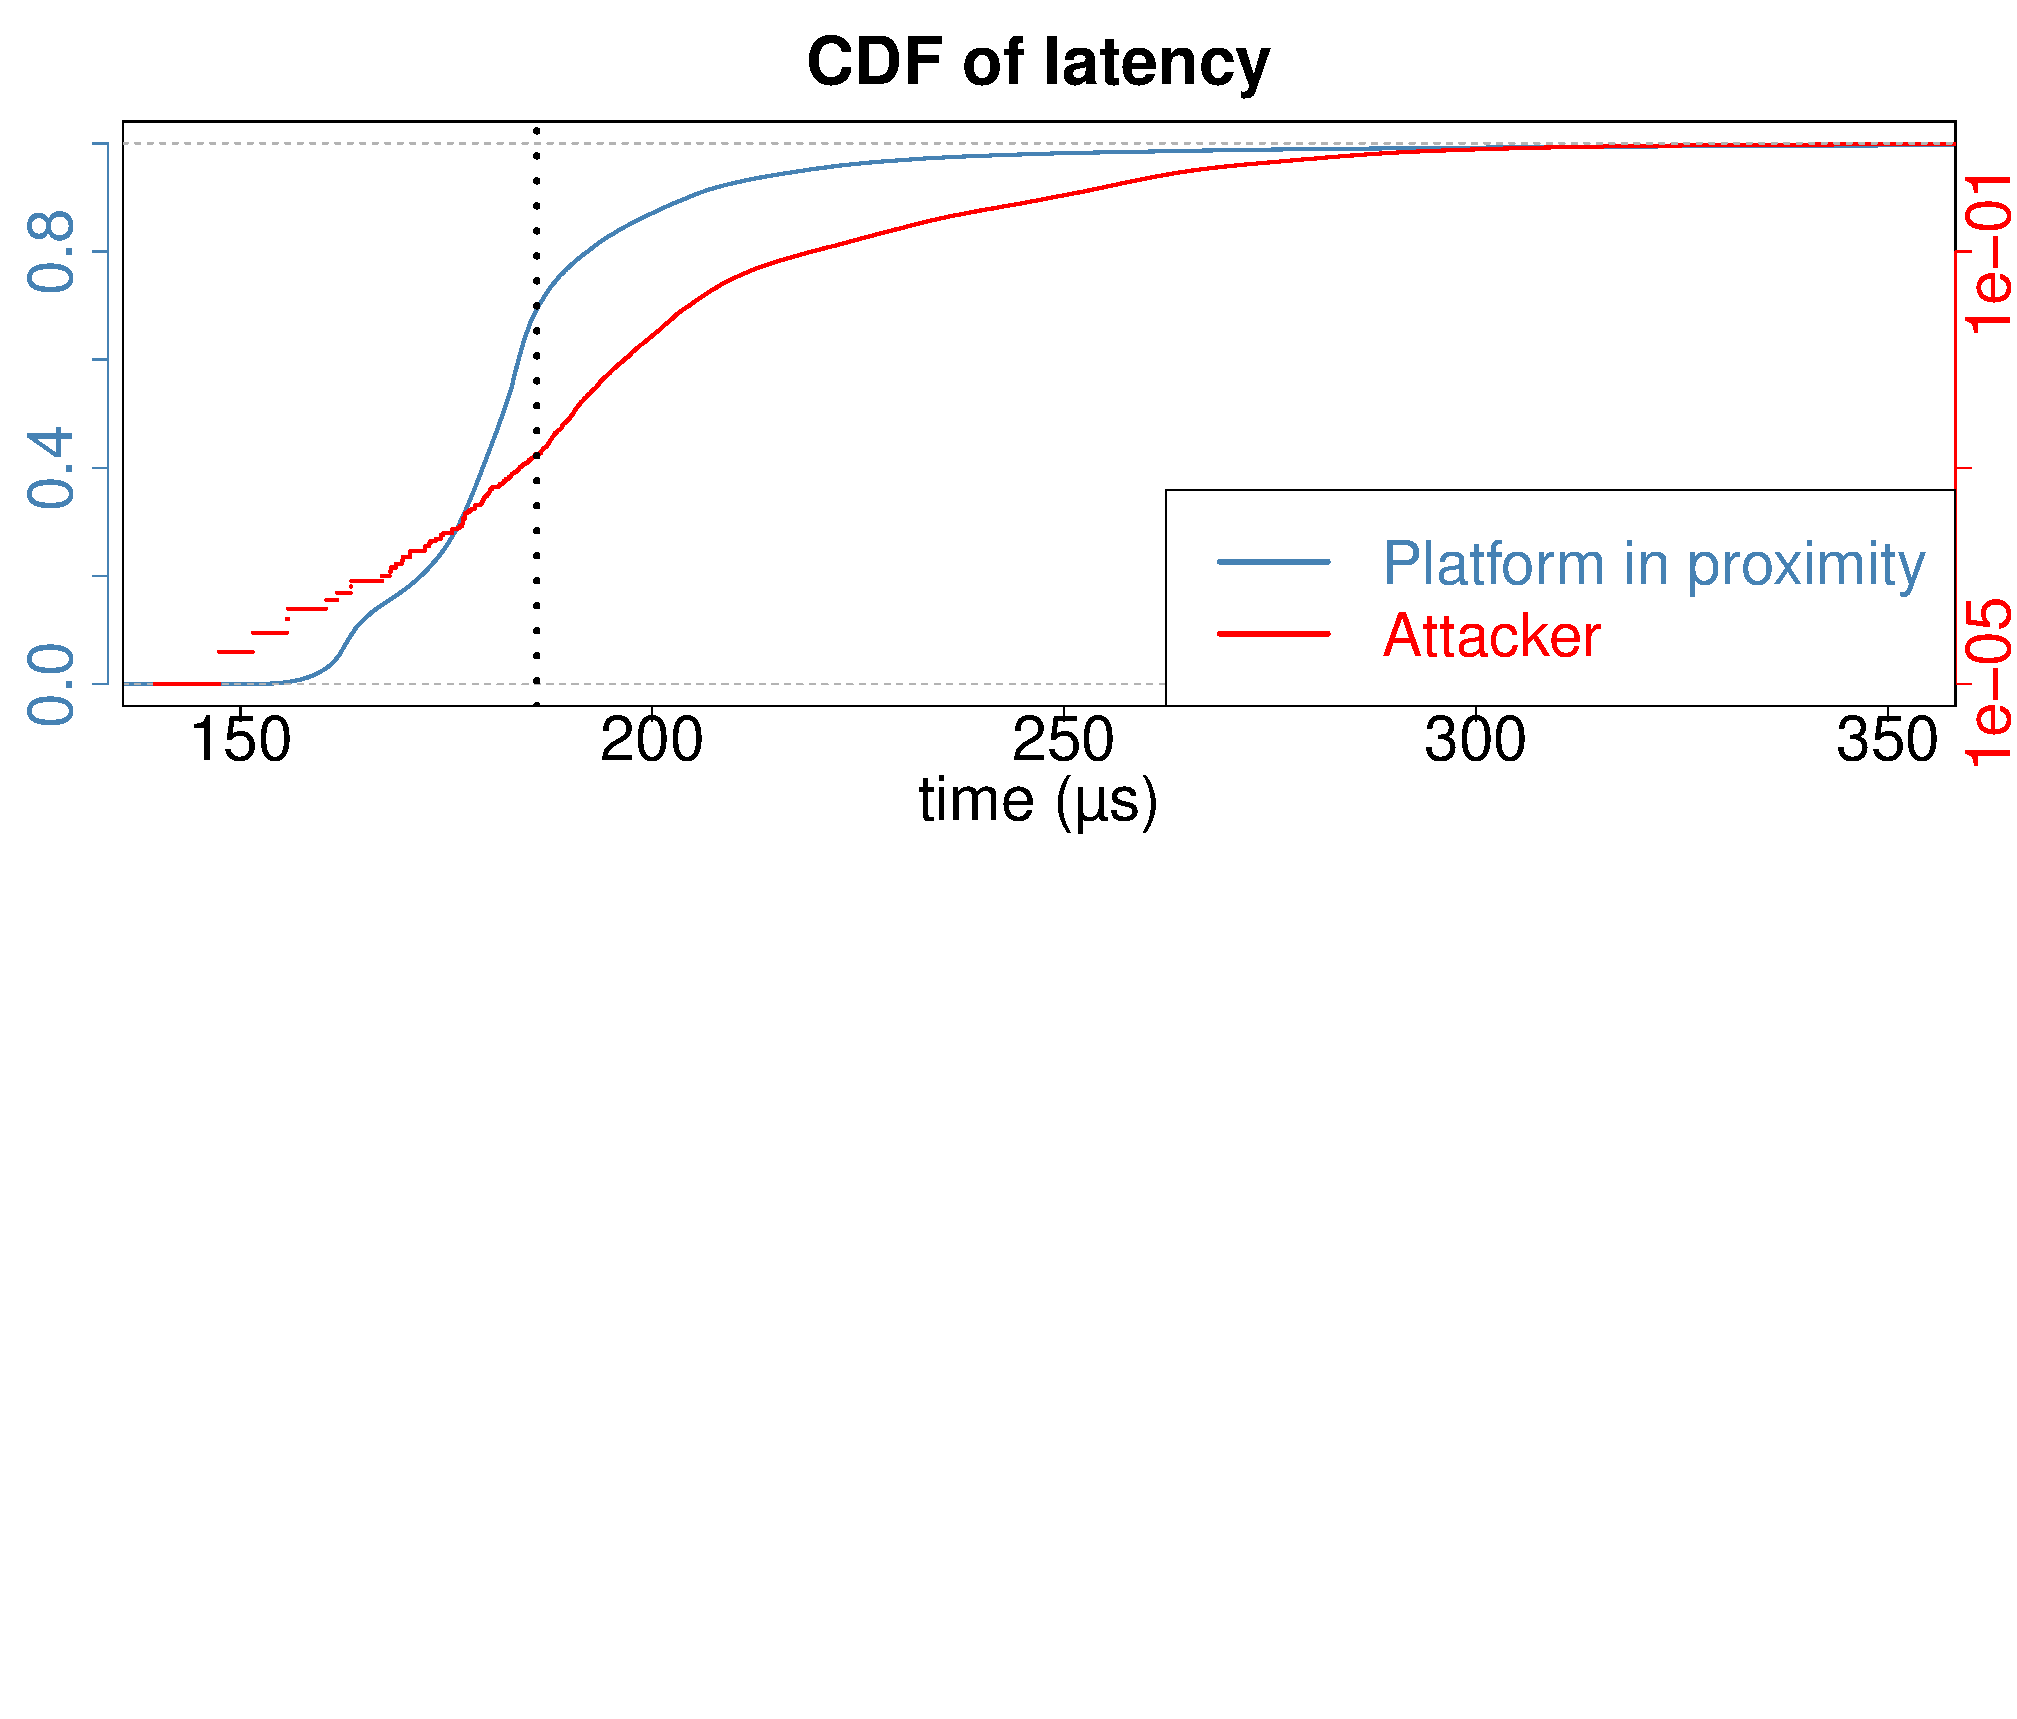
\includegraphics[trim={0 15cm 0 0}, clip, width=0.9\linewidth]{chapters/ProximiTEE/data/fx3_data/CDF_N.pdf}
    \caption[Cumulative distribution function for latencies]{\textbf{Cumulative distribution function for latencies.} We set the threshold \connect at 183 $\mu s$ which has a cumulative probability of $0.693$ in the experiment where no rerouting attack takes place with probability of $1.33\times10^{-4}$.}
    \label{fig:cdf}
\end{figure}


\myparagraph{Choosing a suitable fraction $k$} The next step of the evaluation is to find a suitable fraction $k$ based on the threshold time \connect. Note that both the success probability of the attacker and the legitimate enclave is calculated as the cumulative probability from a binomial distribution (from $nk$ to $n$). Hence, we require to choose a suitable value of $k$ that maximizes $P_{legit}$ while minimizing $P_{adv}$.

We calculate two graphs that are depicted in Figure~\ref{graph:roundSuccess} where the x-axis denotes $k$, and the y-axis denotes attacker's success probability $P_{adv}$ and legitimate success probability $P_{legit}$, respectively, while using \connect$=186 \mu s$. We observe a sharp decrease in the legitimate success probability at $k=0.3$. Hence, fix $k=0.3$ to achieve the maximum $P_{legit}$. Additionally, in the graph of attacker's success probability, the red horizontal line is placed at $10^{-30} \approx 2^{-100}$. Hence we propose to choose any round configuration bellow this horizontal line, where $n \geq 40$. With number of rounds set to $n=50$ and $k=0.3$, we have $P_{legit}=0.(9)_7 7$ and $P_{adv}=3.55\times 10^{-34}$. Similar result could be also observed in Figure~\ref{graph:roundSuccess} where the success probability of the legitimate enclave decreases significantly after $k=0.55$ for \connect$=186\mu s$.



\myparagraph{Generalizing the number of rounds $n$} Figure~\ref{graph:instatAttackerHisto} extends this analysis to the general number of challenge-response rounds spanning from $n=2$ to $100$. Here we compute the probability of attacker returning the reply within $186 \mu s$ for at least $k=0.3$ fraction of challenges. The y-axis denotes the attacker's success probability which diminishes overwhelmingly with the increasing number of challenges (keeping the fraction constant at $k=0.3$). 



\begin{figure}[h]
  \centering
    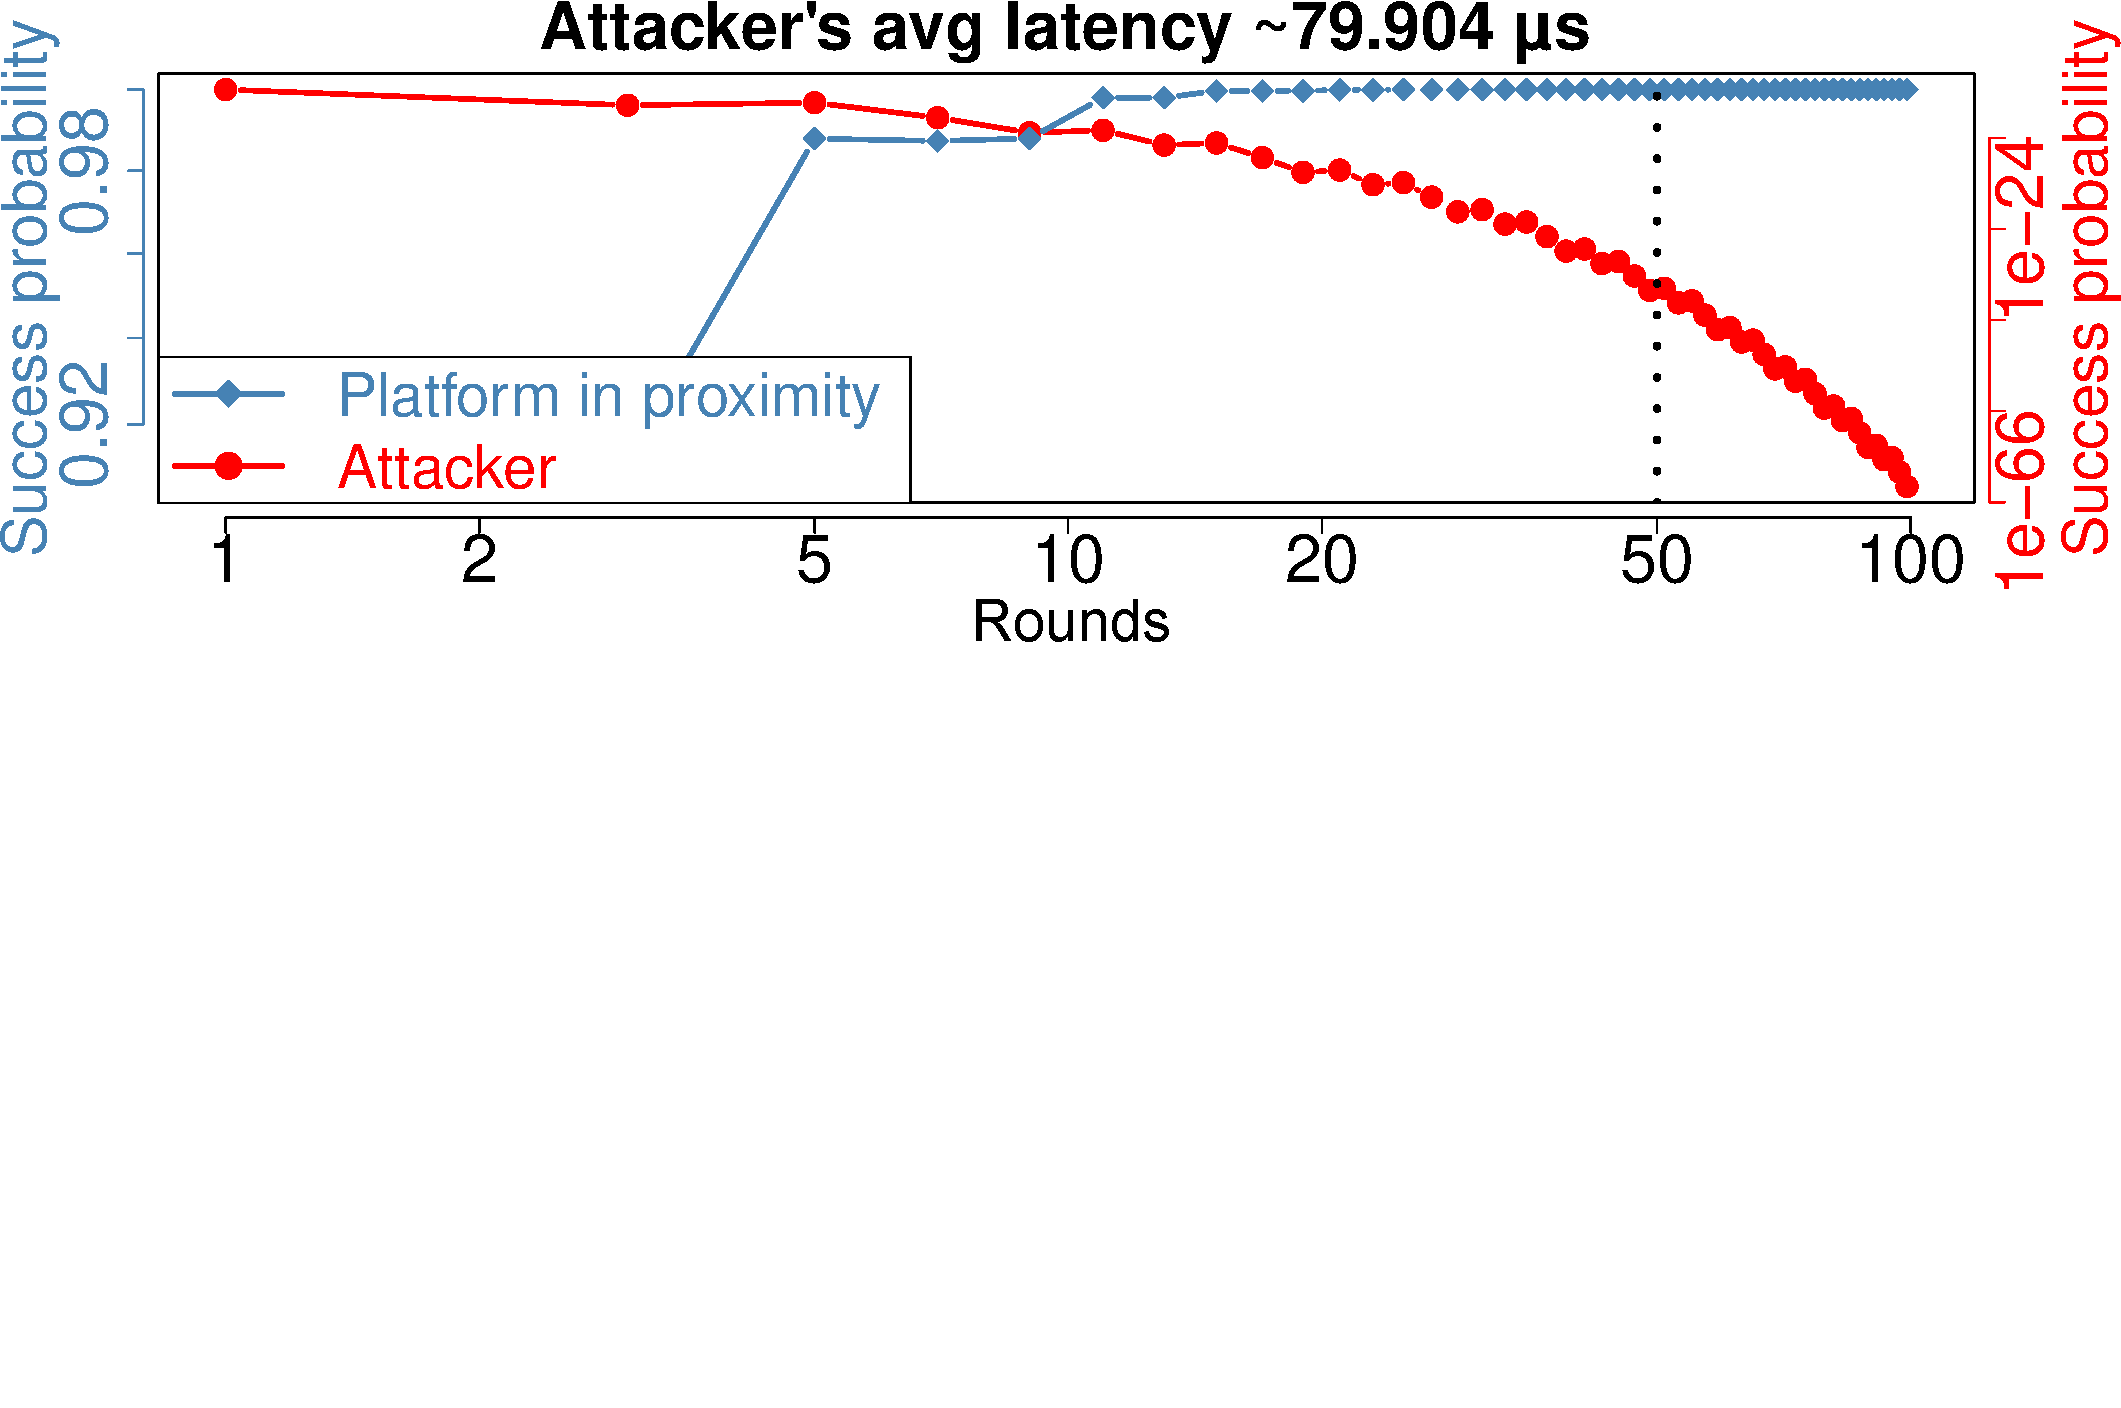
\includegraphics[trim={0 12.8cm 0 0}, clip, width=0.9\linewidth]{chapters/ProximiTEE/figures/InstantAttackerSuccess.pdf}
    \caption[\name distinguishing relay attack]{\textbf{\name distinguishing relay attack.} The figure shows the attacker's success probability $P_{adv}$ and the legitimate success probability $P_{legit}$ for different number of rounds $n$ given a fixed $k$.}

    \label{graph:instantAttackerSuccess}
\end{figure}


\myparagraph{Main result} Figure~\ref{graph:instantAttackerSuccess} shows the legitimate enclave's success probability $P_{legit}$ and the attacker's success probability $P_{adv}$ with different number of rounds. Based on our experiments we set \connect= 186$\mu s$ (see Figure~\ref{graph:instatAttackerHisto}), the threshold fraction $k=0.3$ and the number of rounds $n=50$ which yields a very high legitimate success probability $P_{legit}=0.999999977$ and a negligible attacker's success probability $P_{adv}=3.55\times 10^{-34}$.





\subsection{Periodic Proximity Verification Parameters}
\label{sec:evaluationL:continuousParameters}


For periodic proximity verification we have two main requirements. First, the attacker's success probability $P'_{adv}$ must be negligible. Recall that $P'_{adv}$ refers to an event where the device is detached but the connection is not terminated sufficiently fast. Second, the probability of false positives $P'_{fp}$ should be very low. $P'_{fp}$ refers to an event where the connection is terminated when the device is still attached. Next, we explain the three-step process to set up parameters \detach, $w$ and $f$ for the periodic proximity verification:

\begin{enumerate}
  \item We find out a suitable latency \detach that define the yellow or red round in Figure~\ref{fig:slidingWindow}. The yellow window defines the round of challenge response latency between \connect and \detach, while the red window defines a latency more than \detach. Hence, the probabilities $\Pr[T_{con}\leq \mathcal{L}_{legit}\leq T_{detach}]=\Pr[legit\in\text{yellow}]$, and $\Pr[\mathcal{L}_{legit} \geq T_{detach}]=\Pr[legit\in\text{red}]$ should be very low. $\mathcal{L}_{legit}$ and $\mathcal{L}_{A}$ denote the latency of the legitimate enclave running on the platform in proximity and remote attacker platform's latency respectively.
  \item Based on the threshold \detach, we select a suitable sliding window size $w$ to minimize the attacker success probability $P'_{adv}$ to a negligible quantity.
  \item We fix a suitable frequency $f$ for the periodic challenges. A high $f$ value terminate the communication very fast, leaving very small attacking window.
\end{enumerate}

\myparagraph{Finding suitable threshold \detach} We set the threshold \detach to $510\ \mu s$. We choose this value as we experience zero sample from the timing distribution (refer to the `yellow' distribution Figure~\ref{graph:instatAttackerHisto}) where no rerouting attack takes place. While in the attacker's distribution, the cumulative probability of the response occurring between \connect and \detach is $Pr[$\connect$\leq \mathcal{L}_{A} \leq$\detach$]=\sum_{i=451}^{510}\Pr[\mathcal{L}_{A}=i]=1.4\times10^{-2}$. 
%We account for the experimental error in our model using the standard error of the mean as  $p_e \approx 1.06\times10^{-4}$. The value $p_e$ signifies that a legitimate enclave running on the platform in proximity may take more than 649 $\mu s$ to respond. 
Using \detach, we can now define the challenge response rounds in Figure~\ref{fig:slidingWindow} for a \emph{single round} as following:

\begin{align*}
\Pr[\mathcal{L}_{legit}\leq T_{con}]&=\Pr[legit\in\text{green}]=0.75\\
\Pr[T_{con}< \mathcal{L}_{legit}< T_{detach}]&=\Pr[legit\in\text{yellow}]= 0.237\\
\Pr[\mathcal{L}_{legit}\geq T_{detach}]&=\Pr[legit\in\text{red}]= 7.09\times10^{-3}\\
\Pr[\mathcal{L}_{A}\leq T_{con}]&=\Pr[A\in\text{green}]=9.73\times10^{-5}\\
\Pr[T_{con}< \mathcal{L}_{A}< T_{detach}]&=\Pr[A\in\text{yellow}]= 1.4\times10^{-2}\\
\Pr[\mathcal{L}_{A}\geq T_{detach}]&=\Pr[A\in\text{red}]= 0.985\\
\end{align*} 


\myparagraph{Finding suitable sliding window size $w$} Sliding window size is analogous to that of the number of rounds $n$. We keep  the size of the sliding window as $w=n=50$ as it only requires the \device to remember the past $50$ interactions and achieve high probability for the legitimate enclave and negligible success probability for the attacker. Similar to the previous approach, only if $20$ out of $50$ ($k=0.4$) challenge-response round where responses are within $470\ \mu s$, \name yields success probabilities as the following:

\begin{align*}
 \Pr[A \in \text{success window}]&=P'_{adv} = P'_{fn}= 2.71\times 10^{-67}\\
 \Pr[A \in \text{failed window}]&=\Pr[A\in\text{red}]^2=0.970\\
 \Pr[legit \in \text{success window}]&=0.999999965\\
 \Pr[legit \in \text{failed window}]&=P'_{fp}=\Pr[legit\in\text{red}]^2=5\times10^{-5}
\end{align*}

The probability that a halt window event occurs for a legitimate \app running on the platform in proximity is $\Pr[legit\in\text{red}]\approx 7.09\times10^{-3}$. The \device halts all the data communication to the target platform until the next periodic proximity verification.

If two or more than two latencies $\geq 510\mu s$ (\detach) are received, the \device terminates the connection and revoke the platform. The downtime that can happen as a result of false positive during a connection of 10 years is around $2$ minutes.

\myparagraph{Finding suitable frequency $f$} The frequency $f$ determines how fast the connection is terminated in case the \device device is detached. Note that the \device takes around $12$ $ms$ on average to issue a new random challenge (by reading out the noise of the analog pins of the Arduino board) in the legitimate case. Hence, by performing a round of the protocol as soon as the previous is over, we achieve the maximum attainable average frequency of $\sim83$ rounds per second. We use this frequency as it consumes only $6.48$ KB (0.0011\% of the 
channel capacity) and allows the communication channel to be halted on average after $12 ms$ of the start of a relay attack and terminated in $24 ms$.

\myparagraph{Summarizing the periodic verification results} 
Based on the above strategy, we set the periodic proximity verification parameters as follows: $\Pr[A \in \text{success window}]=P'_{adv} = P'_{fn}= 3.55\times 10^{-34}$, $\Pr[legit \in \text{success window}]=0.999999977$ and $\Pr[legit \in \text{failed window}]=P'_{fp}=\Pr[legit\in\text{red}]^2=1.6\times10^{-4}$ and \detach = $205 \mu s$ (see Figure~\ref{graph:instatAttackerHisto}). If at least two latencies above \detach are received, the \device terminates the connection and revokes the platform. The average downtime due to false positives occurring during a connection of 10 years is around $2$ minutes. 




\subsection{Performance Analysis}

In addition, we evaluated the following two performance metrics:

\begin{enumerate}
  \item \emph{Start-up latency.} The initial proximity verification takes $2$ ms. The complete connection establishment including attestation and \tls handshake takes less than 1 second.  
  


  \item \emph{Operational latency and data overhead.} Our solution adds around $200 \mu s$ of additional latency for \tls and transport over the native \usb interface of the FX3. The data overhead is around 80 bytes per packet for the header and the MAC. Execution of the periodic \name protocol with $83$ rounds/second requires around $156.14$ KBytes/s of data which is only $2.4 \times 10^{-3}$\% of the \usb 3.0 channel capacity. 


\end{enumerate}


\subsection{Additional Experimental Results}


\begin{figure}[t]
  \centering
    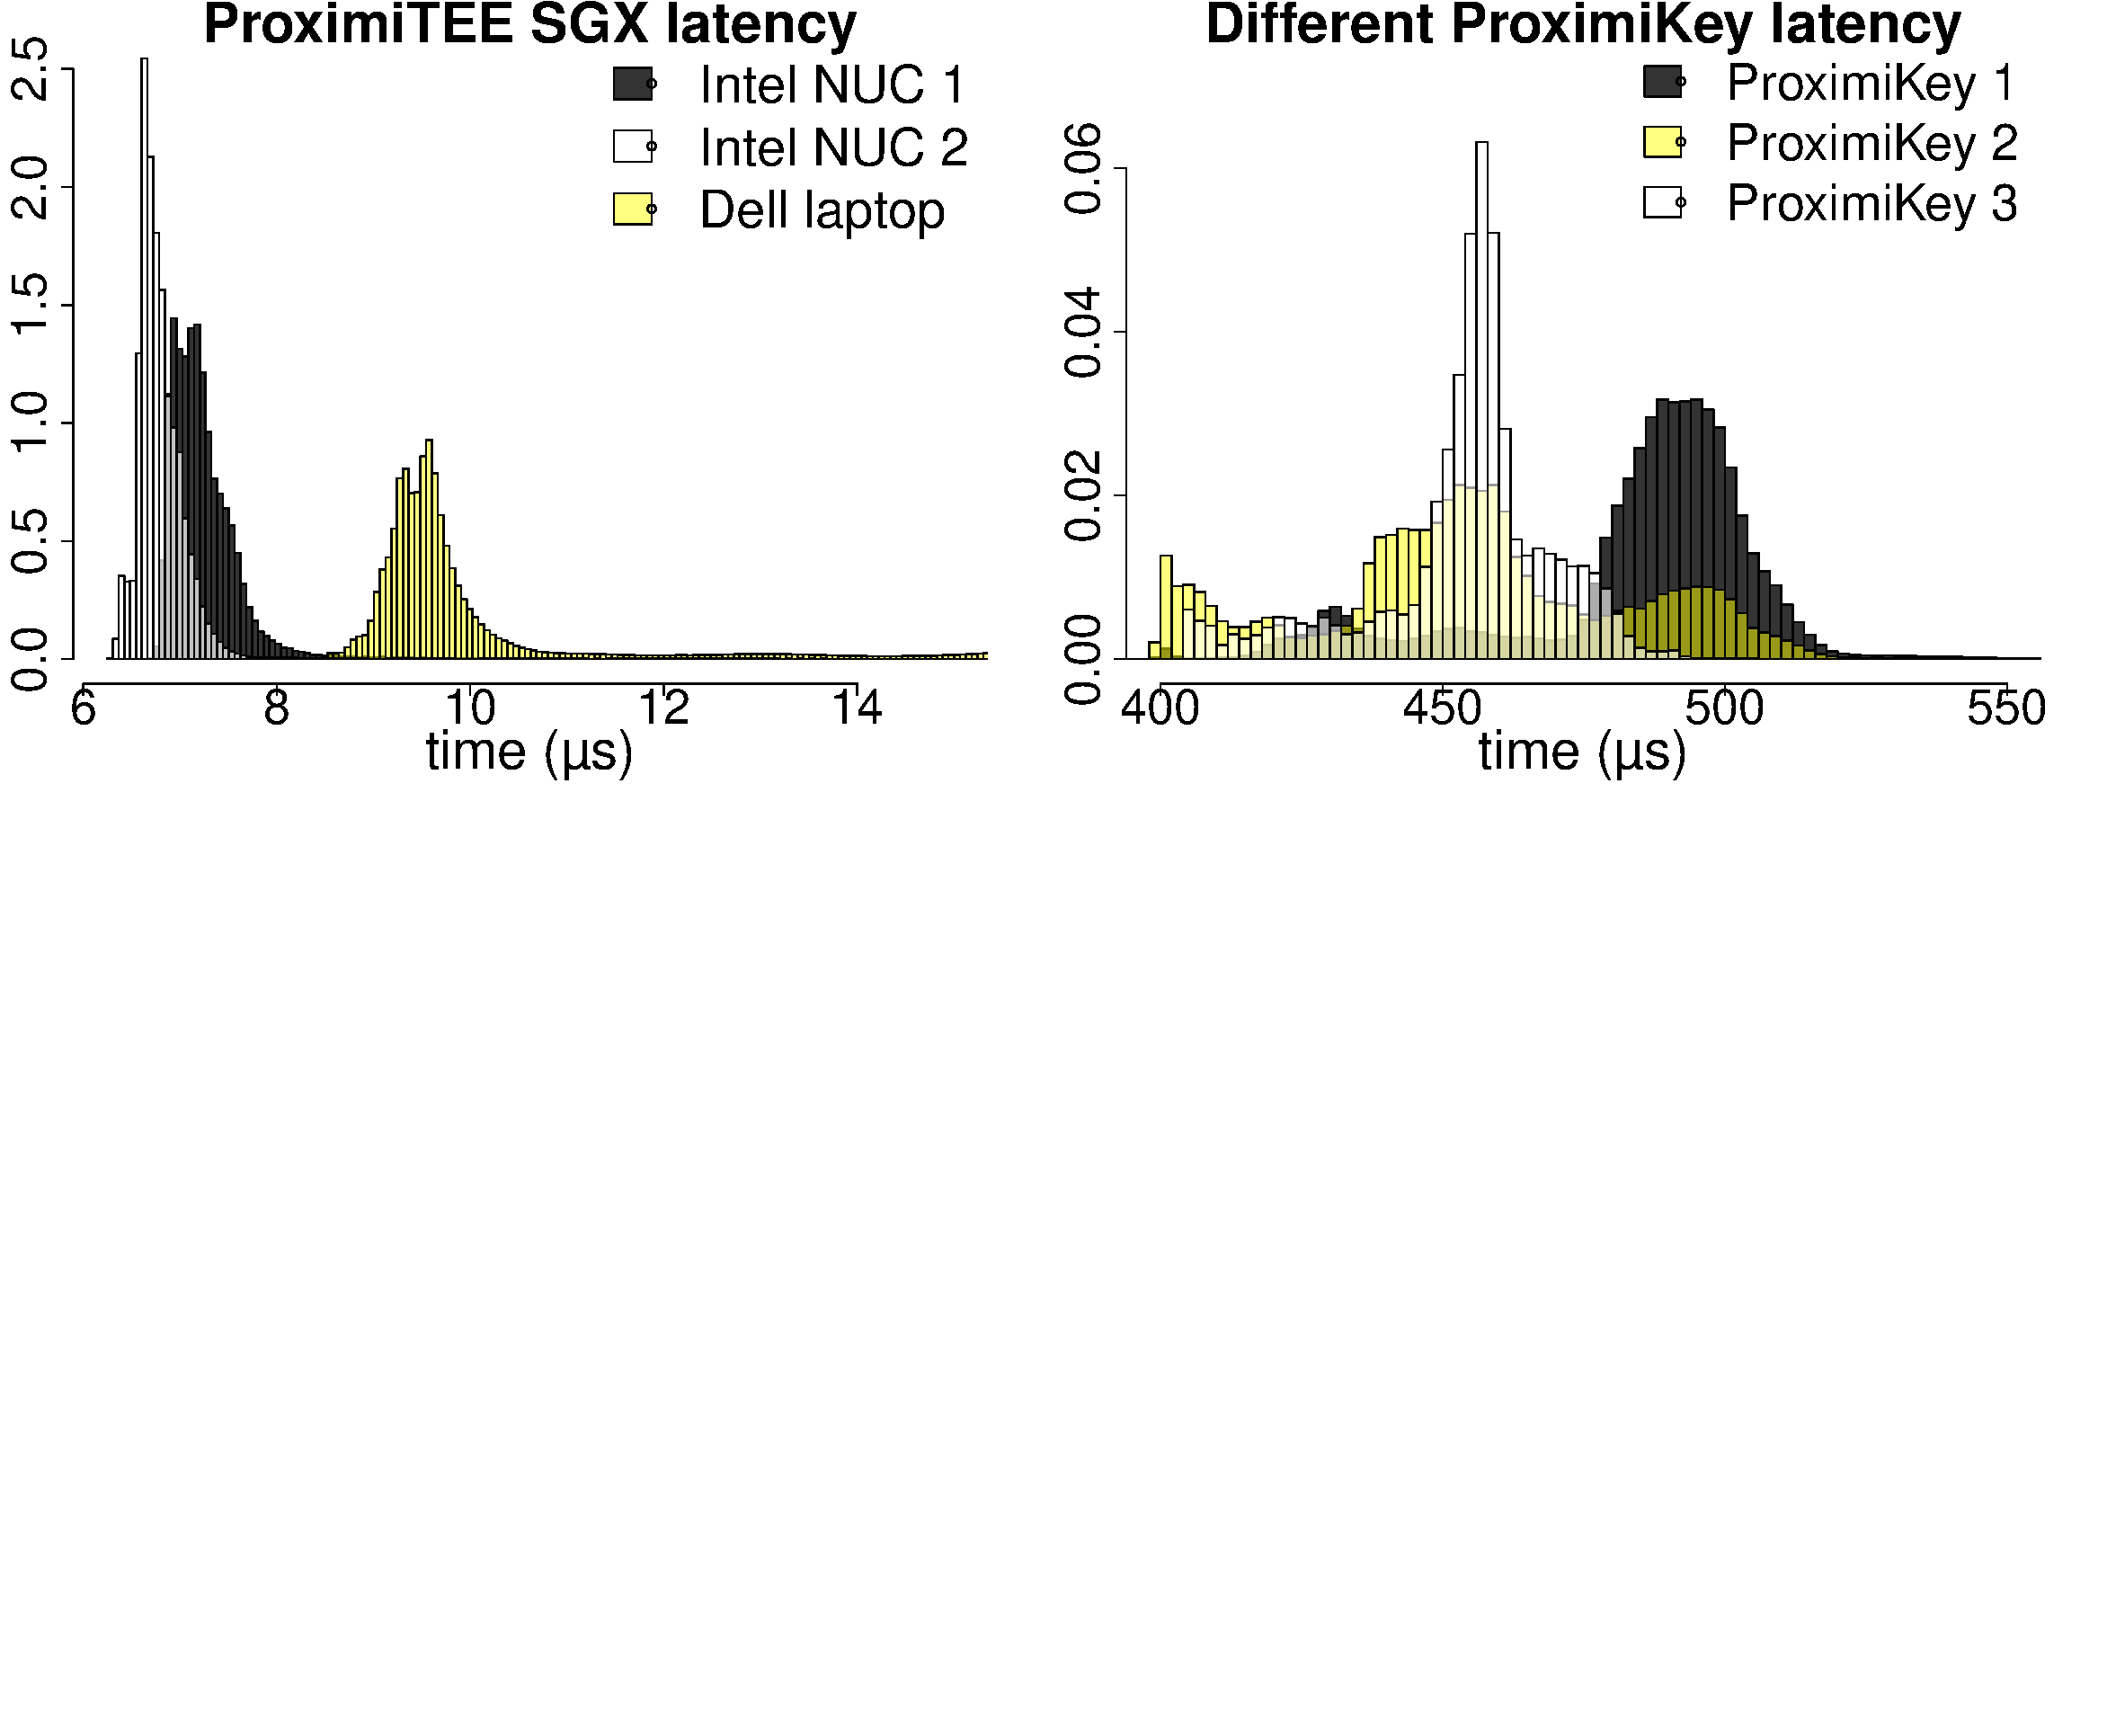
\includegraphics[trim={0 18cm 0 0}, clip, width=\linewidth]{chapters/ProximiTEE/data/graph/PlatformDevice_1.pdf}
    \caption[Effect of different target platforms/\device on the latency.]{\textbf{Effect of different target platforms/\device on the latency.} We evaluates latencies using three different SGX platforms. The Intel NUCs were few microseconds faster. Additionally, we evaluated latencies using three different FX3 boards. The latencies are consistent.}
    %\vspace{-17pt}
    \label{graph:sgxLatency}
\end{figure}

\begin{figure}[t]
  \centering
    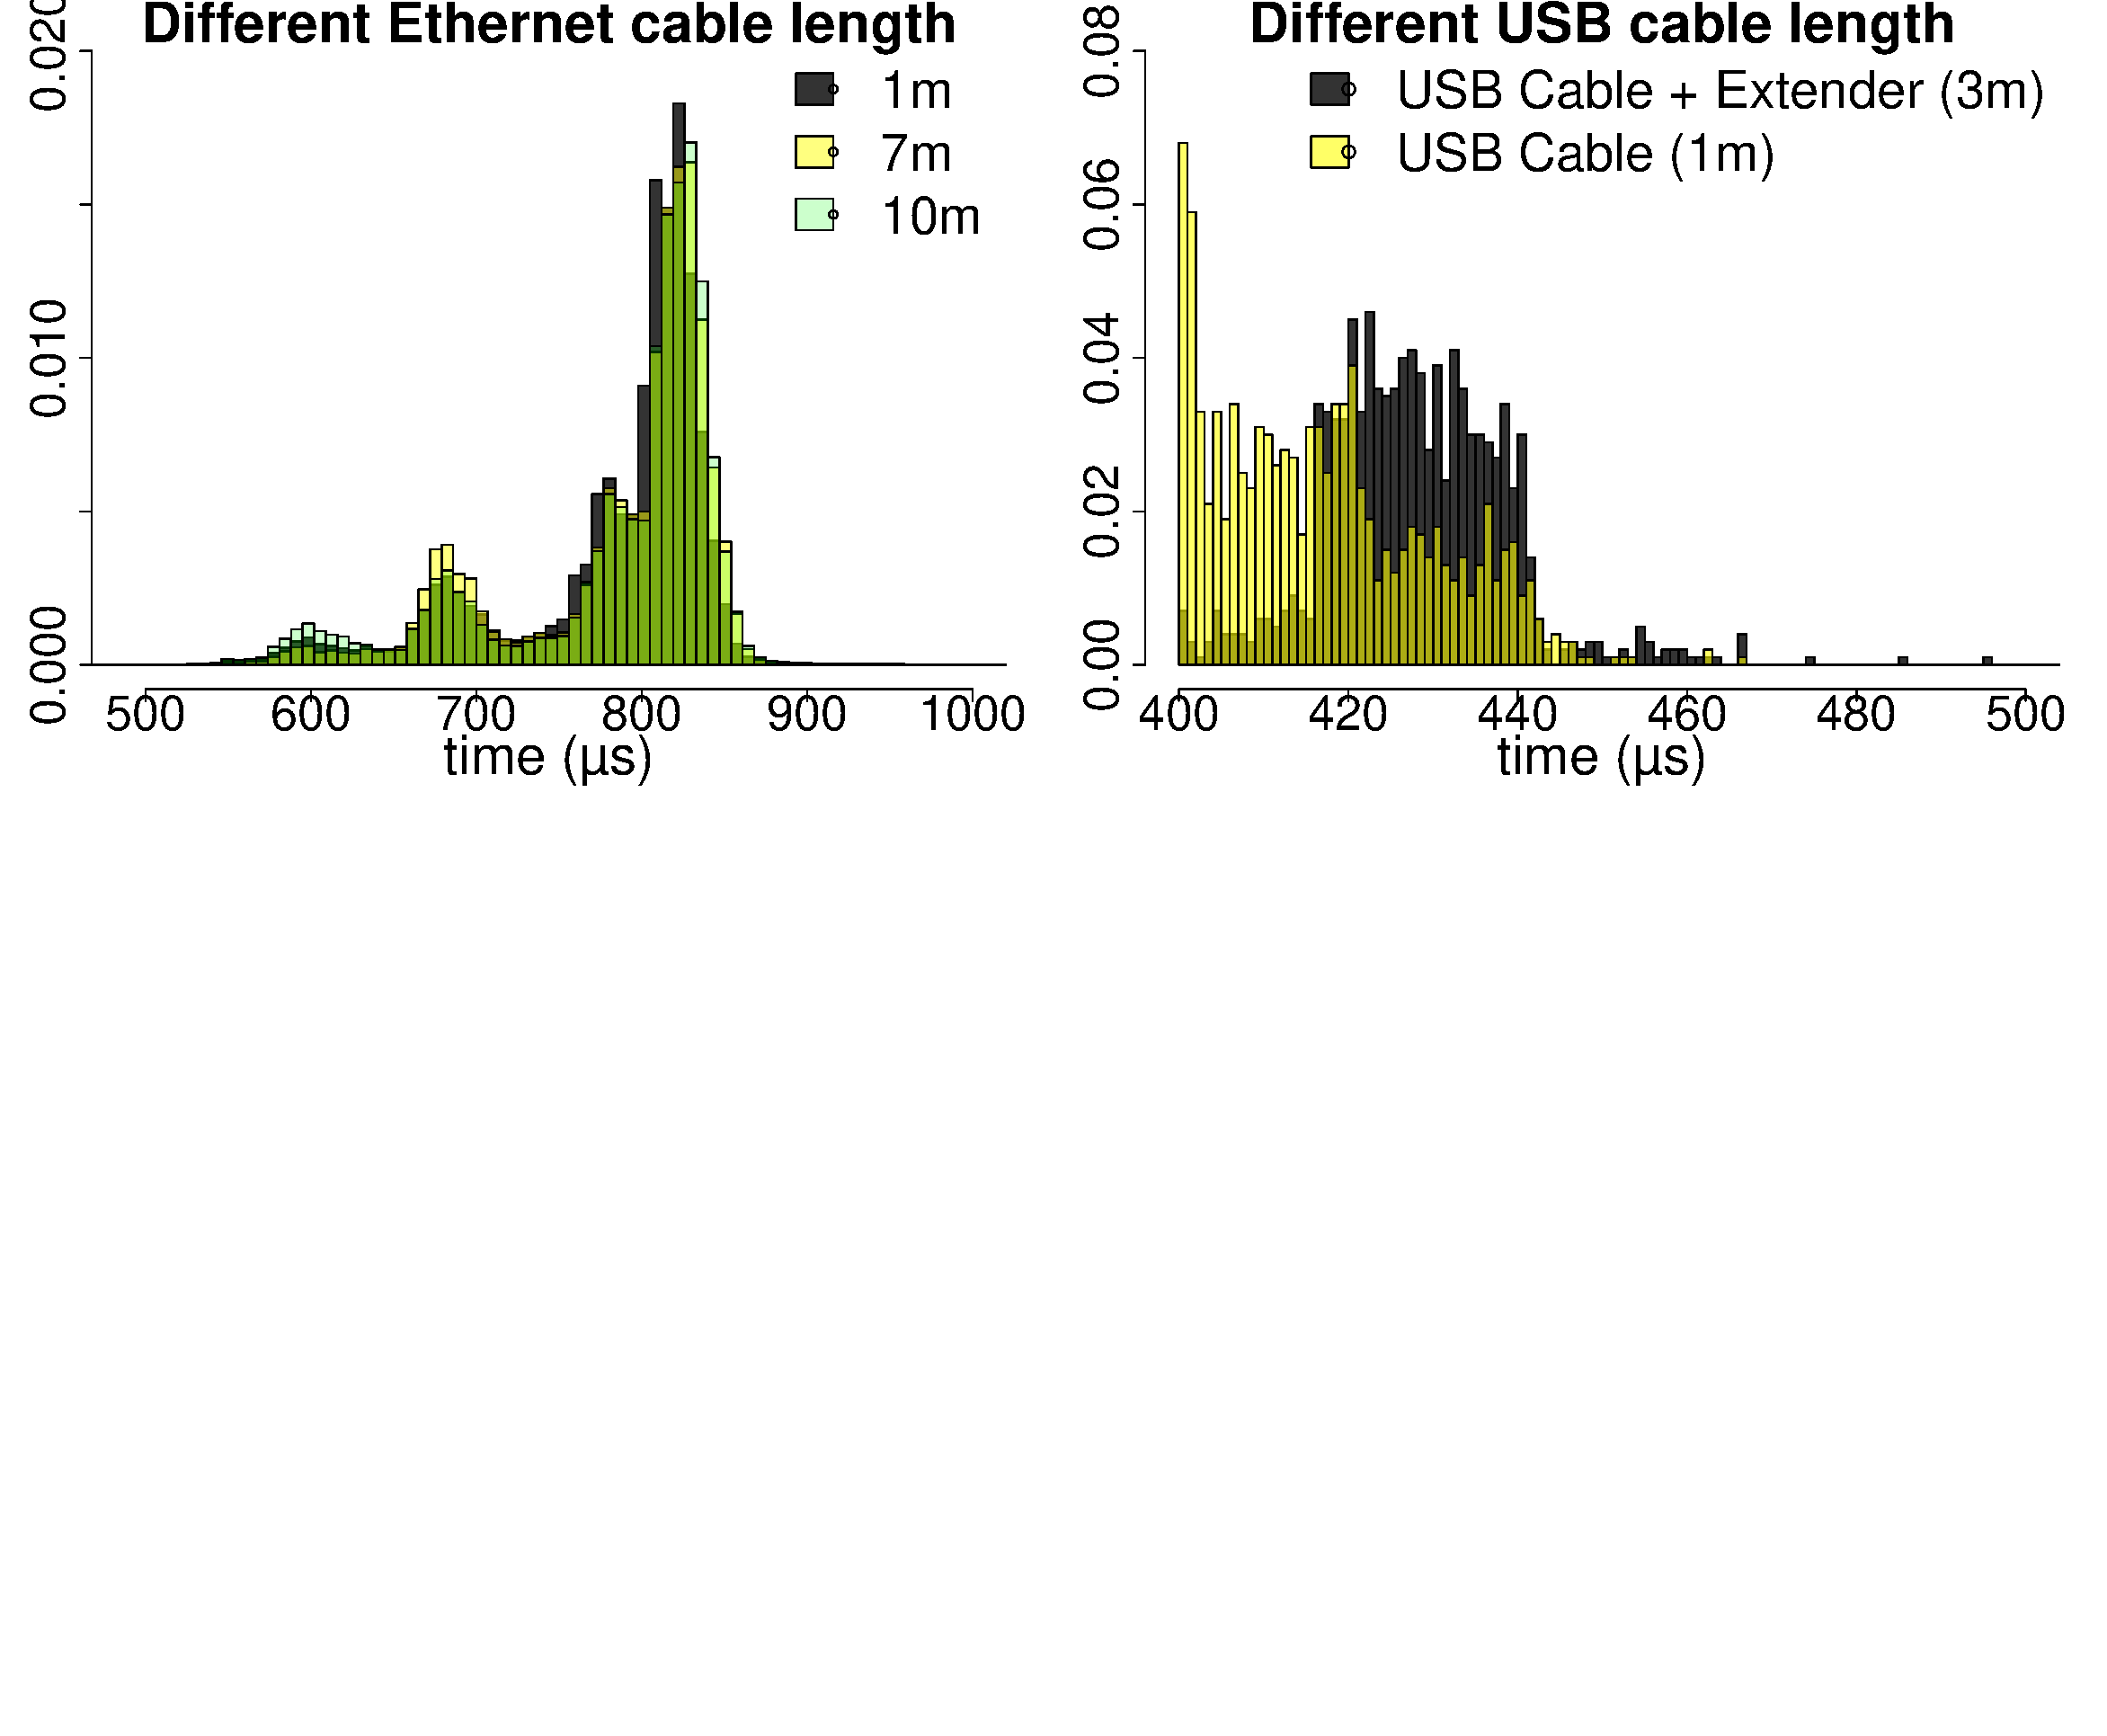
\includegraphics[trim={0 18cm 0 0}, clip, width=\linewidth]{chapters/ProximiTEE/data/graph/CombinedCable_1.pdf}
    \caption[Effect of Different Ethernet/USB cables on the latency]{\textbf{Effect of different Ethernet/USB cables on the latency.} We evaluated latencies two different USB cables: one with an \usb cable (1m) and another with an \usb extender of length 2m attached. Additionally, we evaluated latencies using three different Ethernet cables (1, 7 and 10 m). Latencies are consistent. Note, that the latency is sampled in the experiment conducted with non-\texttt{ping} flood mode.}
    \label{graph:usbCableLength}
\end{figure}


Here we provide results from additional experiments.

We evaluated the consistency of measured latencies across different computing platforms. Figure~\ref{graph:sgxLatency} shows the frequency distribution of latencies across three SGX platforms and three \device devices. We conclude that measurements are consistent result across devices. The two Intel NUCs are few microseconds faster than the Dell Latitude laptop. Additionally, we evaluated the effect of two different \usb cable lengths (3m and 1m) and three different Ethernet cables (lengths of 1m, 7m, and 10m). Figure~\ref{graph:usbCableLength} shows (on the right) that the \usb cable has very small effect on the latency (around 10 $\mu s$ average difference). It also shows (on the left) no significant differences between the different Ethernet cable lengths. 


\begin{figure}[t]
  \centering
    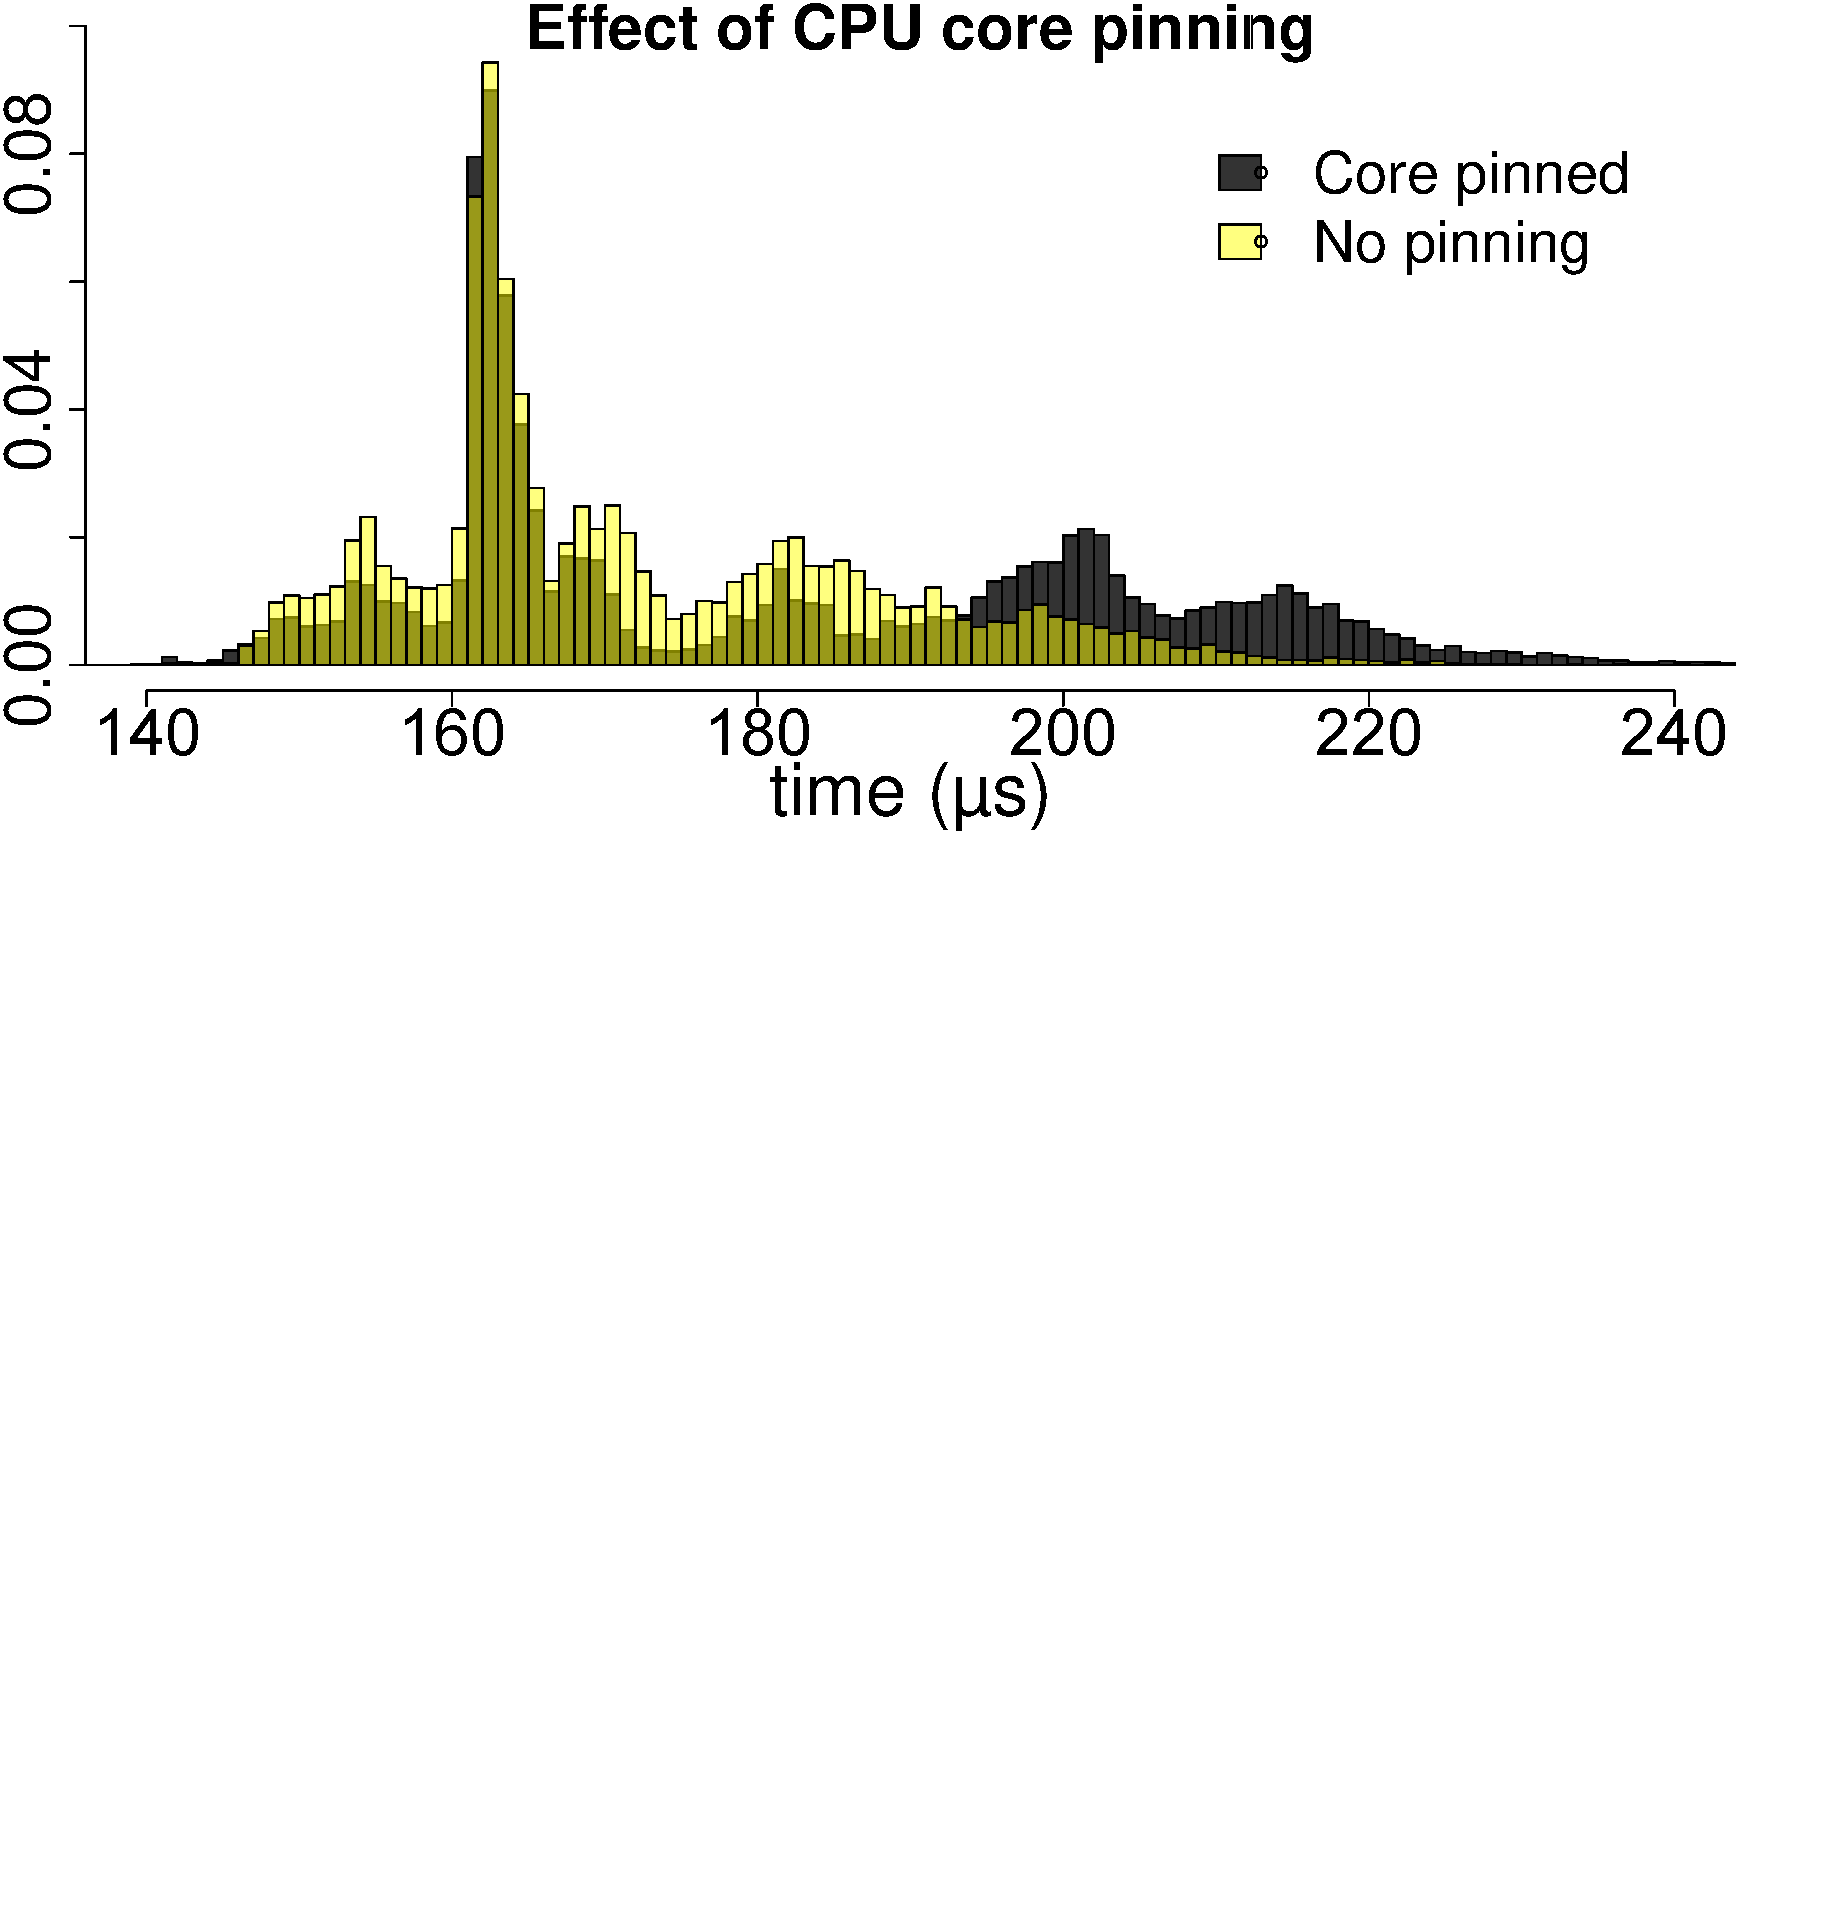
\includegraphics[trim={0 18cm 1.8cm 0}, clip, width=0.75\linewidth]{chapters/ProximiTEE/data/CPU_stress/plot_pin_1.pdf}
    \caption[Effect of CPU core pinning on the enclave application]{\textbf{Effect of CPU core pinning on the enclave application.} Restricting the enclave application to a specific core has a very minor effect on the observed latency.}

    \label{graph:cpuPin}
\end{figure}

\myparagraph{Effects of core pinning} We executes the \name enclave application pinning to specific CPU cores (using the command \texttt{taskset [COREMASK] [EXECUTABLE]}). Core pinning forces the operating system to use a specific set of CPU core(s) to execute a program. CPU pinning may significantly bring down execution time due to the elimination of core switching and ability to reuse L1 and L2 cache. Figure~\ref{graph:cpuPin} illustrates the effect of CPU core pinning vs. no pinning. We experience negligible effect by core pinning. Hence we conclude that the attacker won't gain any advantage by CPU core pinning.

\begin{figure}[t]
  \centering
    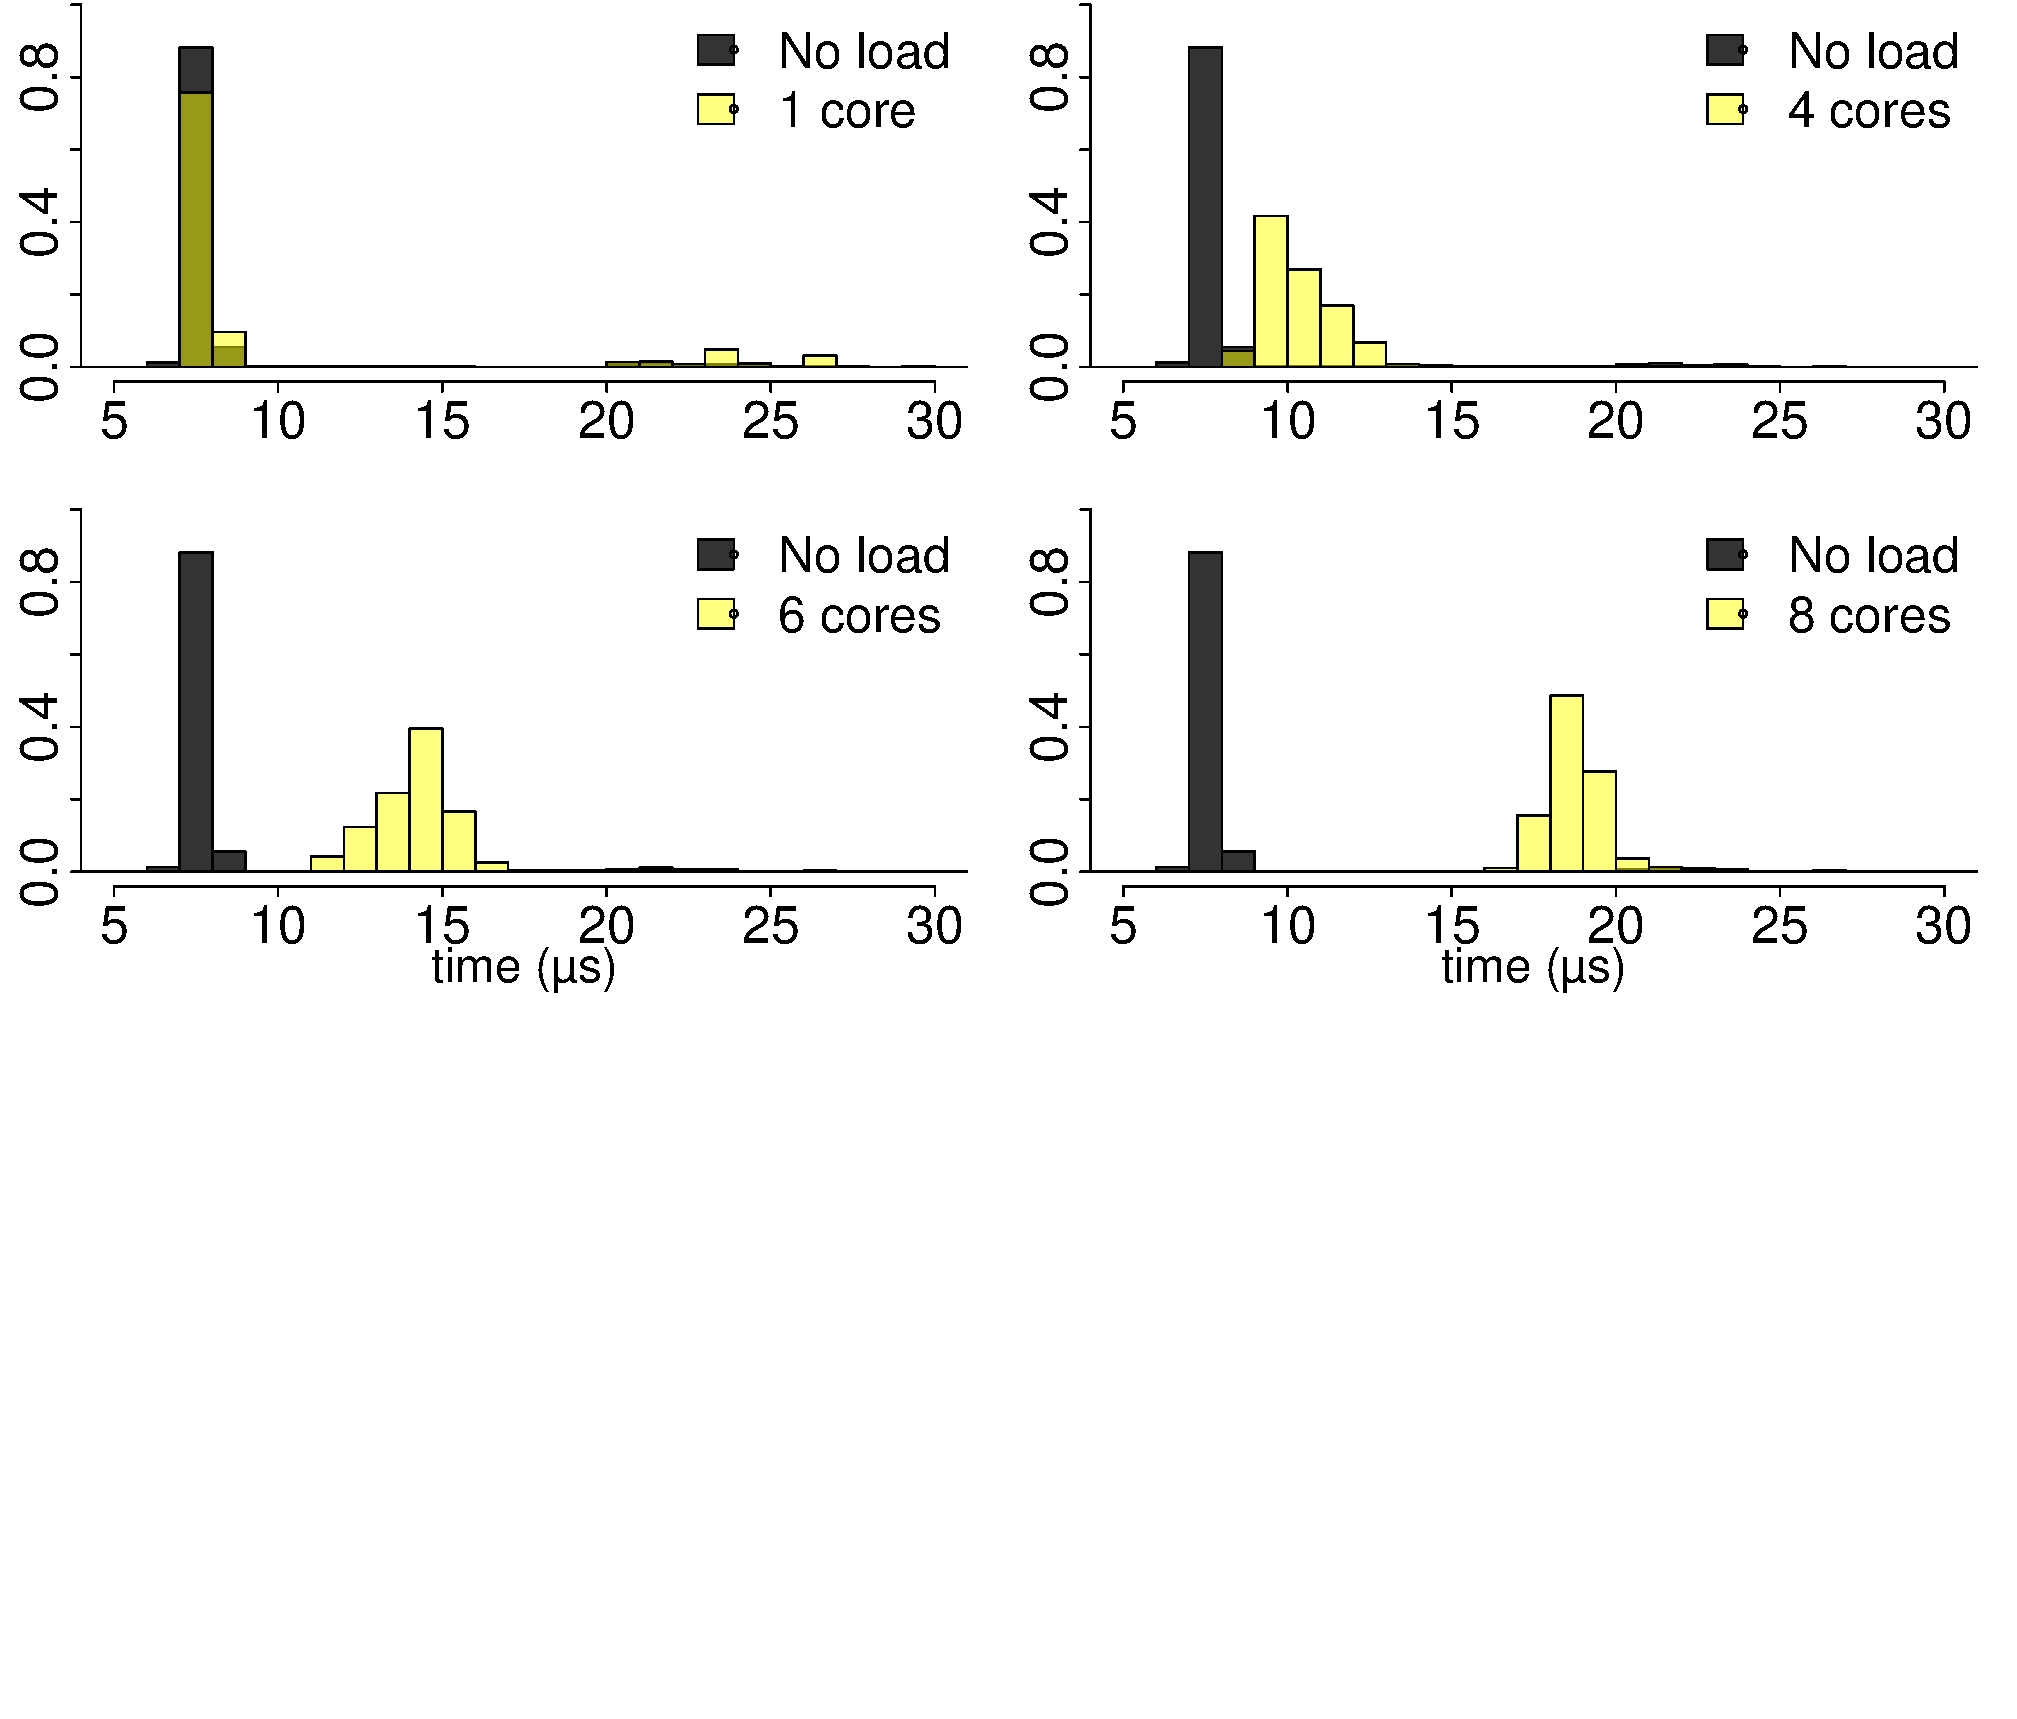
\includegraphics[trim={0 12cm 0 0}, clip, width=0.8\linewidth]{chapters/ProximiTEE/data/CPU_stress/allCore_SGX_1.pdf}
    \caption[Effect on latency experienced by the \device with different number of stressed CPU cores]{\textbf{Effect on latency experienced by the \device with different number of stressed CPU cores.} We evaluated latencies while running CPU intensive benchmark on different number of cores. Note that with higher number of busy cores, the means of the  distributions start to shift towards right but stayed within \connect $= 186\mu s$. We used \texttt{stress-ng} Linux stress-testing application.}
    \label{graph:cpuLoad_SGX}
\end{figure}


\myparagraph{Effects of CPU load} Figure~~\ref{graph:cpuLoad_SGX} shows the enclave execution times with varying degree of CPU stress testing. We used \texttt{stress-ng} to stress different number of CPU cores. We experienced a minor slowdown with the increasing number of busy CPU cores. But the slowdown is insignificant. For example, as shown in the Figure~\ref{graph:cpuLoad_SGX}, we experienced a shift of $12\mu s$ when all the 8 CPU cores are busy executing the benchmark software. Also, note that the load introduced by the benchmark is a sustained load on all the CPU cores which is much more demanding for the CPUs compared to the CPU loads introduced by real-life applications. In that scenarios, the deviation would be even lesser. We conclude that proximity verification for SGX enclaves is reliable even under high system load. In rare cases of extreme system load, proximity verification might fail, but this is an availability concern, not a security threat.


\subsection{Preventing Relay to Co-Located Platform}
\label{sec:co-located}

The main purpose of our experimental evaluation was to show that our inexpensive \name prototype can effectively prevent relay attacks where the adversary redirects the attestation to another platform that is under his physical control in a \emph{different location}. Next, we discuss whether \name can prevent attestation redirection a \emph{co-located} platform, like another server on the same server rack.

If the two co-located platforms are connected through traditional networking technologies like Ethernet (as in our experiments), our evaluation already shows that such relay attacks can be effectively prevented, using a simple and inexpensive embedded device like our prototype. However, in some modern data centers, computing platforms are connected with faster inter-connect technologies like InfiniBand connections that can enable latencies as lows as $7 \mu$s~\cite{liu2003performance}. 

The ability to distinguish relay attacks depends on three key factors. The first is the latency of the channel through which the relay is performed (e.g., $7 \mu$s for InfiniBand). The second is the time required to compute responses to challenges on the target platform (e.g., $6-10 \mu$s in the SGX platforms that we tested). And the third is how much variance the round-trip times between the embedded device and the target platform have (e.g., $10-20 \mu$s in our USB 3.0 prototype). The local communication variance and the response computation time should be less than the relay latency, to enable robust proximity verification. 

We conclude that our simple prototype cannot prevent all possible relays to co-located platforms when very fast inter-connect technologies like InfiniBand are used. To address such relay attacks, one needs a faster and more accurate embedded device that exhibits less variance. For example, PCIe connected FPGAs can have latencies as lows $1 \mu $s~\cite{algoLogic}. Besides better embedded device, one can also increase the number of distance-bounding protocol rounds and reduce the success probability for legitimate attestation $P_{legit}$.


